\chapter{Resultados e Discussão} \label{Resultados e Discussão}

\indent Como forma de otimizar a leitura, os resultados são apresentados e discutidos na sequência. Nesse sentido, a ordem e  numeração apresentados seguem os mesmos adotados na metodologia. Para uma análise  mais detalhada, os resultados se encontram no \href{https://github.com/matheusf30/dengue/tree/main/resultados}{GitHub}, publicados no endereço eletrônico:
\begin{center}
\url{https://github.com/matheusf30/dengue/tree/main/resultados}
\end{center}

\section{Análise Climatológica Espacial}

\indent A tabela \ref{tab:valores_climato} apresenta a análise descritiva das variáveis de temperaturas (mínima, média e máxima) e precipitação acumulada para o Estado de \acrlong{SC}. Ressalta-se que enquanto os valores médios (temperaturas e precipitação) foram calculados para todo o Estado, o que reflete os valores elevados de desvio padrão, os valores mínimos e máximos são os absolutos da série.

\indent Em se tratando de temperatura média diária, o menor valor que a série histórica do Estado de \acrlong{SC} apresentou foi de -4,4 C, sendo 1,6 C para dados semanais. O valor máximo da temperatura média foi de 37,5 C, dados diários, e 34,9 C, dados semanais. A média diária da temperatura mínima para o Estado foi de 18,3 C, tanto para valores diários quanto semanais, e o desvio padrão foi de 4,8 C e 4,2 C, dados diários e semanais, respectivamente. 

\indent Com relação a temperatura mínima absoluta diária, o menor valor que a série histórica do Estado de \acrlong{SC} apresentou foi de -8,3 C, sendo -2,8 C quando agrupado semanalmente. O valor máximo absoluto da temperatura mínima foi de 30,3 C, dados diários, e 25,0 C, dados semanais. A média diária da temperatura mínima para o Estado foi de 14,3 C, sendo o mesmo valor quando agrupado em semana, e o maior desvio padrão de 4,9 C para dados diários. O desvio padrão semanal foi de 4,1 C. Esse resultado mínimo foi encontrado por \citeonline{Guerra2023Regionalizacao} como anomalia para o Planalto Sul catarinense durante os dias de inverno. "Os \ingles{outliers} mostram que as temperaturas marcaram valores abaixo de -5 C em eventos extremos durante este período" \cite{Guerra2023Regionalizacao}.  

\indent Ao analisar os valores mínimos absolutos de dados diários, percebe-se a distribuição nos seguintes municípios para as temperaturas mínima, média e máxima, respectivamente: Anitápolis, Arroio Trinta e Alto Bela Vista. O município de Anitápolis está localizado na parte serrana da Grande Florianópolis. Na mesorregião Oeste, localizam-se os municípios de Alto Bela Vista (microrregião de Concórdia) e Arroio Trinta (microrregião de Joaçaba), este apresenta altitude acima de 800 metros. Observado por \citeonline{Guerra2023Regionalizacao}, em regiões mais elevadas, observam-se temperaturas menores com extremos mais intensos.

\begin{table}[htbp]
    \begin{center}
    \caption{Valores médio, desvio padrão em relação a média, mínimo e máximo absoluto das variáveis climatológicas no Estado de \acrlong{SC} na série histórica (2000-2023).}
    {\rowcolors{1}{lightgray}{white}
    \begin{tabular}{r|cccc}
    \hline
    \toprule
    \rowcolor{darkgray} \textcolor{white}{Variável Climatológica} & \textcolor{white}{Média} & \textcolor{white}{Desvio Padrão} & \textcolor{white}{Mínima} & \textcolor{white}{Máxima}\\
    \midrule
    Temperatura Mínima Diária (C) & 14,3 & 4,9 & -8,3 & 30,3\\
    Temperatura Mínima Semanal (C) & 14,3 & 4,1 & -2,8 & 25,0\\
    Temperatura Média Diária (C) & 18,3 & 4,8 & -4,4 & 37,5\\
    Temperatura Média Semanal (C) & 18,3 & 4,2 & 1,6 & 34,9\\
    Temperatura Máxima Diária (C) & 24,1 & 5,4 & -1,6 & 41,0\\
    Temperatura Máxima Semanal (C) & 24,1 & 4,5 & 7,6 & 38,3\\ 
    Precipitação Diária (mm) & 4,3 & 12,9 & 0,0 & 292,6\\
    Precipitação Semanal (mm) & 30,2 & 41,5 & 0,0 & 519,2\\
    \bottomrule
    \label{tab:valores_climato}
    \end{tabular}}
    \end{center}

    \small{Fonte: Elaboração própria (2024).}
\end{table}

\indent Para a temperatura máxima diária, o menor valor foi de -1,6 C, sendo 7,6 C para dados semanais. O valor máximo da temperatura máxima foi de 41,0 C, dados diários, e 38,3 C, dados semanais. A média diária da temperatura máxima para o Estado de \acrlong{SC} foi de 24,1 C, tanto para valores diários quanto semanais, e o desvio padrão foi de 5,4 C e 4,5 C, dados diários e semanais, respectivamente.

\indent O município de Xanxerê, na região Oeste, apresentou os maiores valores máximos absolutos de registros diários para as temperaturas mínima e máxima. O maior valor máximo absoluto para a temperatura média foi registrado em Vitor Meireles, localizado no alto vale do rio Itajaí. De acordo com \citeonline{Guerra2023Regionalizacao}, "as maiores temperaturas são observadas nas áreas litorâneas e no oeste do estado".

\indent Ainda observado por \citeonline{Guerra2023Regionalizacao}, a região Oeste catarinense apresenta dias como temperaturas extremas, acima de 35 C, durante o período de verão. Nesse mesmo período de verão, a região litorânea pode apresentar extremos próximos a 40 C. Esse fato ocorre antecipadamente no Meio Oeste, apresentando extremos de temperatura diária acima de 35 C durante a primavera, principalmente entre setembro e outubro \cite{Guerra2023Regionalizacao}.

\indent Todas as temperaturas apresentaram comportamento semelhante, mínima, média e máxima, por compartilharem o mesmo método de agrupamento semanal, baseado na média dos dias da semana. Logo, tem-se valores de máximas e mínimas próximos a média quando agrupados semanalmente e os valores de médias diárias e semanais são semelhantes, por conta do próprio método. Essa suavização por agrupamento também é verificada no desvio padrão, sendo menor em dados semanais. 

\indent A precipitação na série histórica de \acrlong{SC} obteve seu maior valor em 292,6 mm diários e 519,2 mm semanais (acumulado de sete (7) dias). O fato de  \acrlong{SC} passar por períodos de estiagens, foi registrado o menor valor de zero (0) mm também no valor absoluto mínimo semanal. A média de precipitação para o Estado é de 4,3 mm diários e 30,2 mm semanais, tendo 12,9 mm e 41,5 mm como desvio padrão para dados diários e semanais, respectivamente.

\indent Os valores máximos absolutos de precipitação foram observados em Águas Mornas, dados diários, e Águas de Chapecó, acumulado semanal. O município de Águas Mornas se encontra no início da região serrana da Grande Florianópolis, enquanto o município de Águas de Chapecó se localiza na região Oeste. "Enquanto no Extremo Oeste e Oeste o pico chuvoso ocorre na primavera, nas áreas litorâneas e em grande parte dos Planaltos predominam as chuvas de verão" \cite{Guerra2023Regionalizacao}.

\indent "Os maiores índices pluviométricos anuais são registrados no Oeste, Grande Florianópolis e Litoral Norte. Por outro lado, no Litoral Sul, [...], os totais anuais de precipitação são os menores" (\acrlong{SC}, \citeyear{AtlasSCnatureza}). Para a região do Oeste, \cite{Guerra2023Regionalizacao} tem observado acumulados maiores de precipitação durante a primavera.

\indent Para as séries diária e semanal, os valores mínimos absolutos são semelhantes, zero (0) mm, pois há períodos em que não precipita em regiões de \acrlong{SC} por mais de sete (7) dias. Esse valor também diz respeito a característica do dado, sendo uma variável quantitativa de razão, em contraposição às temperaturas, que são variáveis quantitativas intervalares.

\indent Para os dados semanais, o município de Bom Jardim da Serra, no Planalto Sul, apresentou os valores mínimos absolutos para ambas as temperaturas (mínima, média e máxima). Assim como o município de Tunápolis, na região Oeste, apresentou os valores máximos absolutos para ambas as temperaturas (mínima, média e máxima).

\indent A distribuição média anual das variáveis entomo-epidemiológicas e climatológicas é apresentada na figura \ref{fig: distribuicao_sazonal_SC_total}. Percebe-se que tanto para focos de \latim{Aedes} sp. quanto para casos de dengue há concentrações regionalizadas, principalmente: Oeste Catarinense, nas proximidades dos municípios de Chapecó e Concórdia; Norte Catarinense, com especial destaque para o município de Joinville; Vale do Itajaí, nas proximidades dos municípios de Itajaí e Blumenau; e Grande Florianópolis.

\indent Parte do comportamento entomo-epidemiológico observado no presente estudo acompanha o comportamento climático das temperaturas citado por \citeonline{Guerra2023Regionalizacao}, que também observou regionalização nos maiores valores observados; assim como a regionalização da precipitação (figura \ref{fig: distribuicao_sazonal_SC_total}).

\indent A espacialização da temperatura também é influenciada por sistemas meteorológicos em associação com o diferencial de altitude entre planícies, planaltos e serras catarinenses (figura \ref{fig: tmin_mapa_coropletico_sazonal_se_total}, \ref{fig: tmed_mapa_coropletico_sazonal_se_total} e \ref{fig: tmax_mapa_coropletico_sazonal_se_total}). Como exposto na figura \ref{fig: prec_mapa_coropletico_sazonal_se_total}, os maiores índices pluviométricos anuais são registrados nas regiões Oeste, Grande Florianópolis e Litoral Norte (\acrlong{SC}, \citeyear{AtlasSCnatureza}).

\newpage
\begin{citacao}
"Ao tratar-se de temperaturas, os efeitos da continentalidade são claros nos valores observados e em seus ciclos diurnos [...]. Os resultados mostram que as maiores temperaturas são observadas nas áreas litorâneas e no oeste do estado..." \cite[pg-152]{Guerra2023Regionalizacao}.
\end{citacao}

\indent Em uma análise espacial de imagens termais no município de Itajaí, \citeonline{Matiola2019Avaliacao} verificou áreas com temperaturas mais elevadas onde, nessas mesmas áreas, havia ocorrência de focos do mosquito \latim{Aedes aegypti}. \citeonline{Matiola2019ANALISE} chamam atenção para o comportamento que ocorre entre as variáveis climatológicas e entomológicas em Chapecó durante a primavera austral, onde não há um ciclo bem marcado entre verão e outono, como normalmente é encontrado na literatura.

"A flutuação populacional de \latim{A. aegypti}, em Chapecó, mantém um padrão de aumento no crescimento nos  meses  mais  quentes,  diminuindo nos  meses  mais  frios,  indicando  assim,  relação  da  infestação com a sazonalidade \cite{Matiola2019ANALISE}.

\indent A figura \ref{fig:distribuicao_sazonal}, apresentada na seção \ref{sazonal} (Análise Climatológica de Municípios Selecionados), mostra a distribuição sazonal de todas as variáveis. Essa distribuição seguiu cronologicamente as semanas epidemiológicas. Dessa maneira, há concordância temporal entre os elementos climatológicos (precipitação e temperaturas mínima, média e máxima) e variáveis entomológicas (focos de \latim{Aedes} sp.) e epidemiológicas (casos de dengue).

\begin{landscape}
\begin{figure}[htbp]
    \begin{center}
    \caption{Distribuições de médias anuais de variáveis entomo-epidemiológicas (focos de \latim{Aedes} sp. e casos de dengue) e climatológicas (precipitação e temperaturas mínima, média e máxima) em Santa Catarina.}
    \label{fig: distribuicao_sazonal_SC_total}
    \subfloat[Casos de Dengue \label{fig: casos_mapa_coropletico_sazonal_se_total}]{
        \centering
        \includegraphics[width=0.5\textwidth]{figuras/casos_mapa_coropletico_sazonal_se_total_dissertacao.png}
        }
    \subfloat[Focos de \latim{Aedes} sp. \label{fig: focos_mapa_coropletico_sazonal_se_total}]{
        \centering
        \includegraphics[width=0.5\textwidth]{figuras/focos_mapa_coropletico_sazonal_se_total_dissertacao.png}
        }
    \subfloat[Precipitação (mm) \label{fig: prec_mapa_coropletico_sazonal_se_total}]{
        \centering
        \includegraphics[width=0.5\textwidth]{figuras/prec_mapa_coropletico_sazonal_se_total_dissertacao.png}
        }\hfill
    \subfloat[Temperatura Mínima (C) \label{fig: tmin_mapa_coropletico_sazonal_se_total}]{
        \centering
        \includegraphics[width=0.5\textwidth]{figuras/tmin_mapa_coropletico_sazonal_se_total_dissertacao.png}
        }
    \subfloat[Temperatura Média (C) \label{fig: tmed_mapa_coropletico_sazonal_se_total}]{
        \centering
        \includegraphics[width=0.5\textwidth]{figuras/tmed_mapa_coropletico_sazonal_se_total_dissertacao.png}
        }
    \subfloat[Temperatura Máxima (C) \label{fig: tmax_mapa_coropletico_sazonal_se_total}]{
        \centering
        \includegraphics[width=0.5\textwidth]{figuras/tmax_mapa_coropletico_sazonal_se_total_dissertacao.png}
        }\hfill
    \end{center}
    \small{Fonte: Elaboração própria (2024).}
\end{figure}
\end{landscape}

\section{Análise Climatológica de Municípios Selecionados} \label{sazonal}

\indent Visando uma análise regionalizada das variáveis entomo-epidemiológicas e climatológicas foram selecionadas  quatro (4) municípios de \acrlong{SC}: Florianópolis, Itajaí, Joinville (localizados na região litorânea) e Chapecó (região oeste). Essa seleção foi realizada também por estes apresentarem maior frequência e volume de dados, além de representarem municípios populosos e características regionais distintas.

\indent Em primeira análise, é possível perceber na figura \ref{fig:distribuicao_sazonal} que os picos de casos de dengue são atingidos algumas semanas epidemiológicas após os valores máximos de ambas as temperaturas (máxima, mínima e média), apresentando um hiato de 10 a 15 semanas entre esses picos (máximos de temperaturas seguidos dos picos de casos).

\indent Esses máximos valores de casos de dengue também precedem os mínimos registros de ambas as temperaturas, com hiato entre cinco (5) e 10 semanas epidemiológicas. Esse fato corrobora o comportamento sazonal da doença, ocorrendo com maior incidência durante as semanas epidemiológicas do outono austral. Ainda durante o inverno no hemisfério sul, pode-se perceber uma redução nos focos de \latim{Aedes} sp (figura \ref{fig:distribuicao_sazonal}).

\indent No município de Chapecó, em especial, percebe-se adiantamento da curva de casos de dengue (figura \ref{fig:distribuicao_sazonal_CHA}), como observado por \citeonline{Guerra2023Regionalizacao} com o comportamento climatológico da temperatura, apresentando extremos que superam 35 C em setembro e outubro.

\begin{citacao}
"As estações de transição mostram valores intermediários, mas também é um período de grande amplitude térmica e com uma grande quantidade de \ingles{outliers}. No outono se observam desvios expressivos de frio, que se aproximam de zero grau ejá em abril, possivelmente associado a episódios de frio antecipado. Na primavera se destacam os extremos de calor fora de época, que superam até mesmo os observados no verão, com temperaturas que superam os 35 C em setembro e outubro" \cite[pg-113]{Guerra2023Regionalizacao}.
\end{citacao}

\begin{figure}[htbp]
    \begin{center}
    \caption{Distribuições de sazonalidade de variáveis entomo-epidemiológicas (focos de \latim{Aedes} sp. e casos de dengue) e climatológicas (precipitação e temperaturas mínima, média e máxima) para os municípios de Florianópolis, Itajaí, Joinville e Chapecó; \acrlong{SC}.}
    \label{fig:distribuicao_sazonal}
    \subfloat[Florianópolis \label{fig: distribuicao_sazonal_FLO}]{
        \centering
        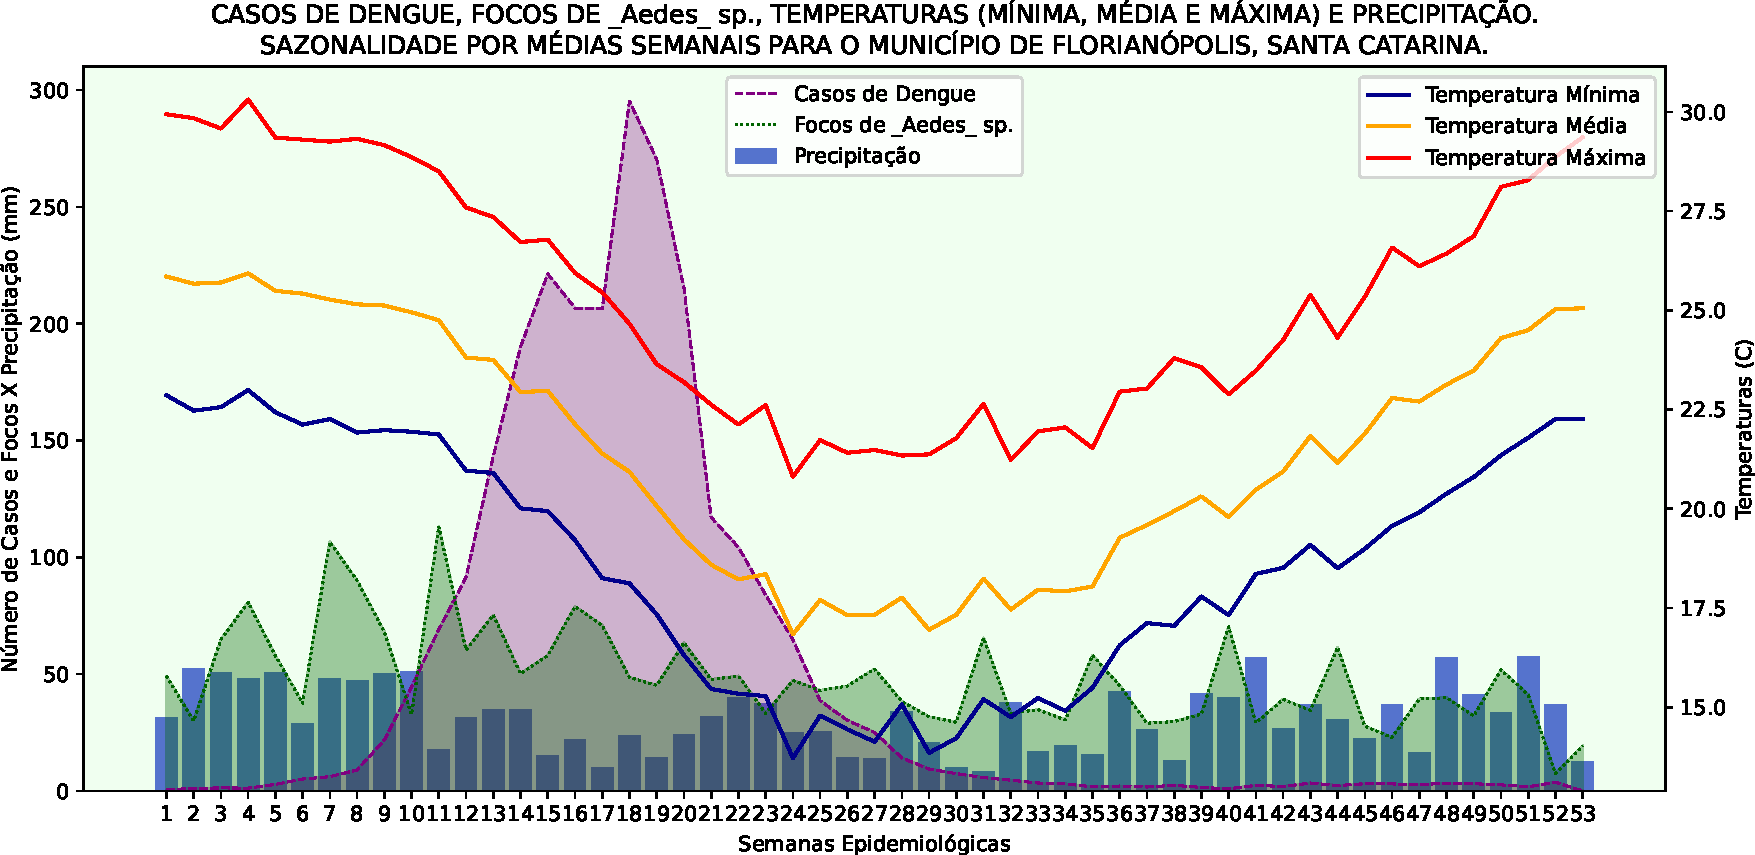
\includegraphics[width=0.5\textwidth]{figuras/distribuicao_sazonalidade_semanal_FLORIANOPOLIS.pdf}
        }
    \subfloat[Itajaí \label{fig: distribuicao_sazonal_ITA}]{
        \centering
        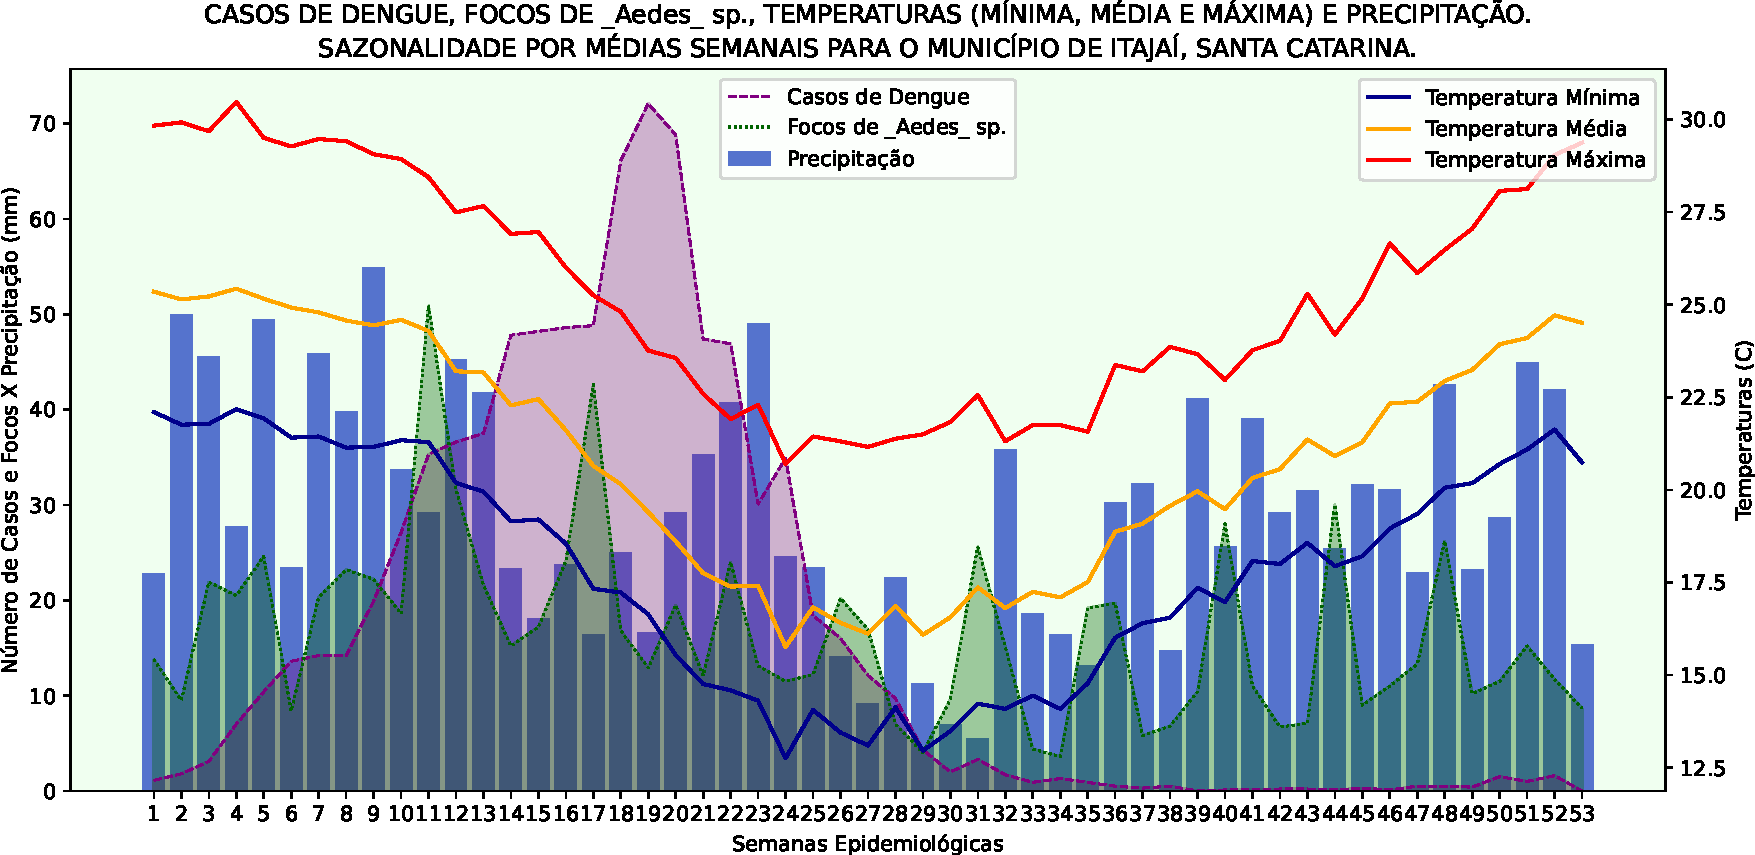
\includegraphics[width=0.5\textwidth]{figuras/distribuicao_sazonalidade_semanal_ITAJAI.pdf}
        }\hfill
    \subfloat[Joinville \label{fig: distribuicao_sazonal_JOI}]{
        \centering
        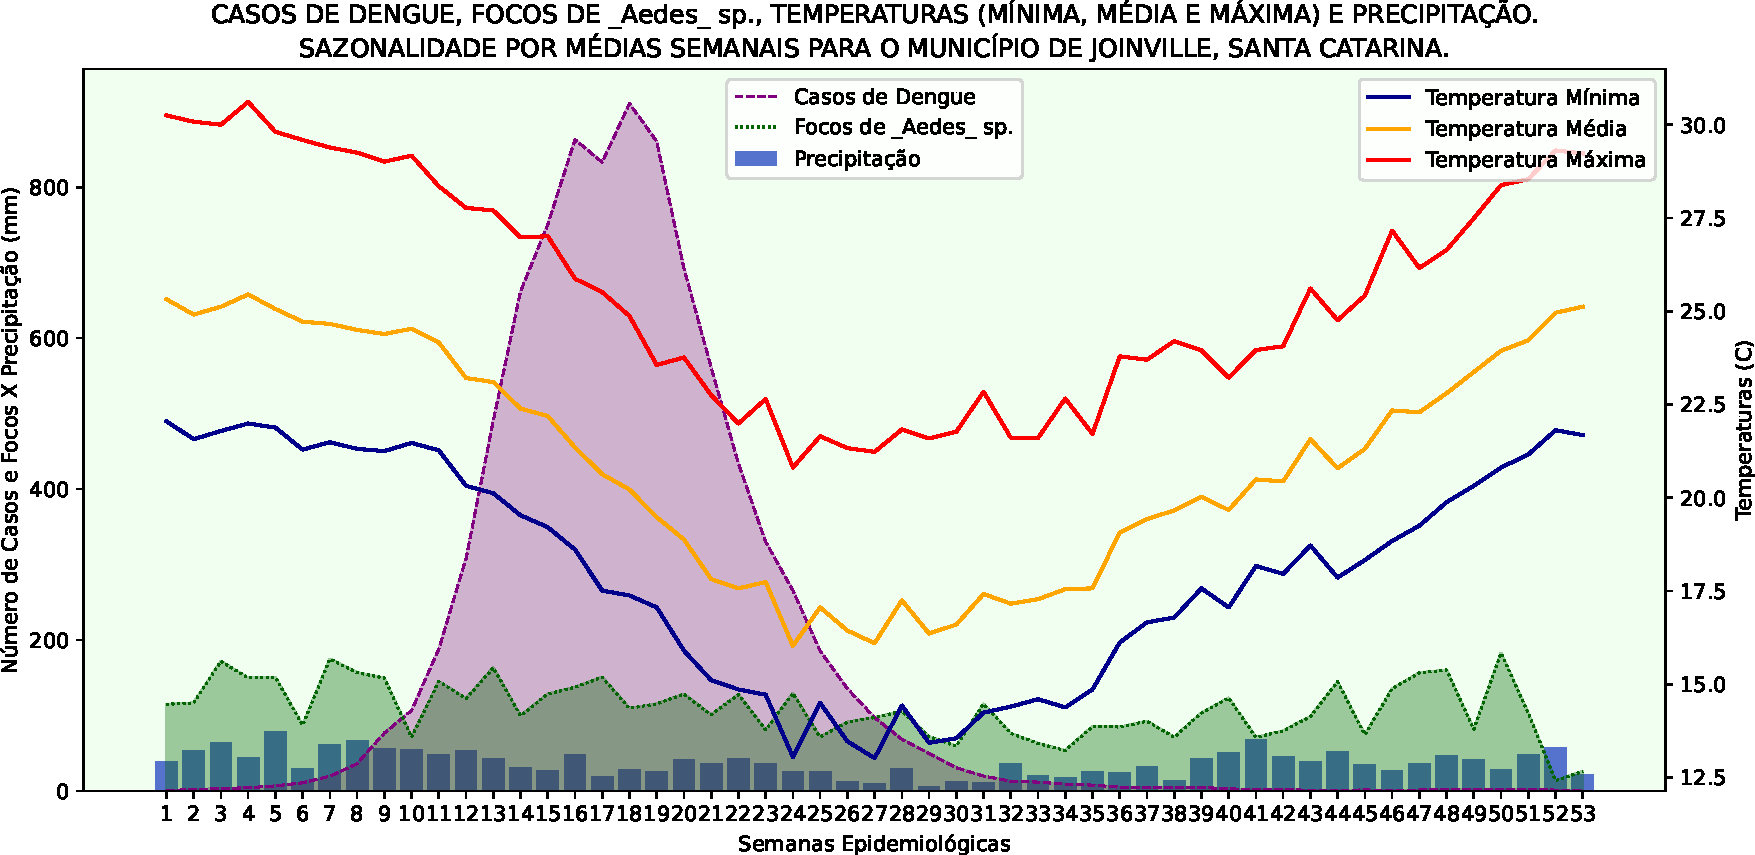
\includegraphics[width=0.5\textwidth]{figuras/distribuicao_sazonalidade_semanal_JOINVILLE.pdf}
        }
    \subfloat[Chapecó \label{fig:distribuicao_sazonal_CHA}]{
        \centering
        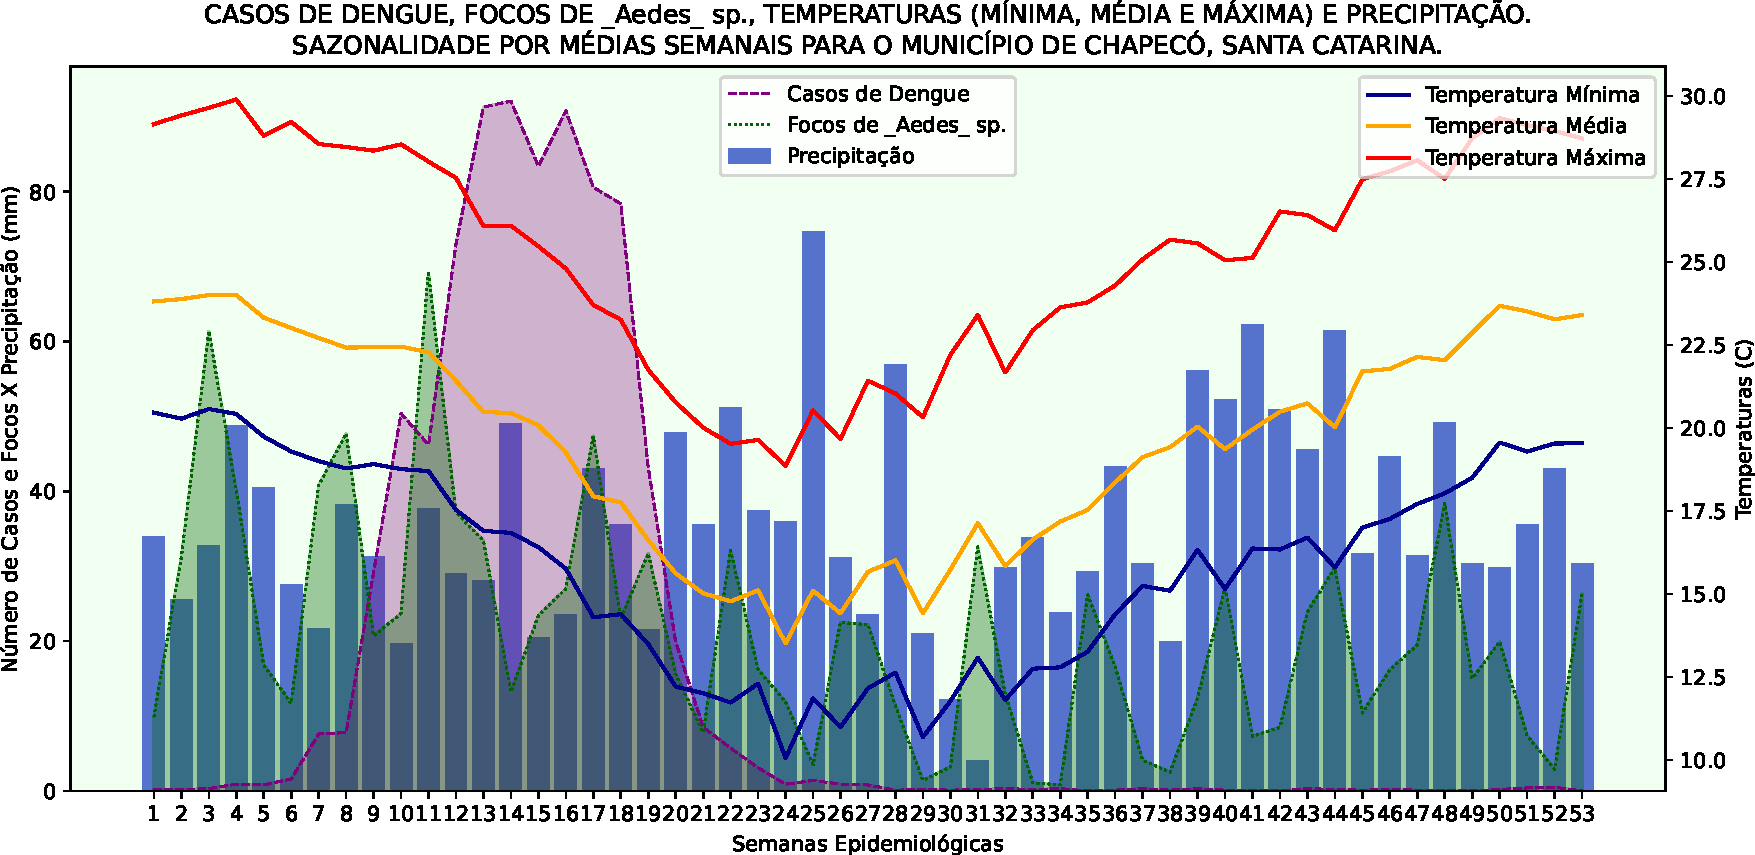
\includegraphics[width=0.5\textwidth]{figuras/distribuicao_sazonalidade_semanal_CHAPECO.pdf}
        }\hfill
    \end{center}
    \small{Fonte: Elaboração própria (2024).}
\end{figure}

\indent A partir desse padrão observado, selecionou-se semanas epidemiológicas, especialmente entre a décima primeira (11ª) e a vigésima segunda (22ª) semanas. Sendo as seis (6) primeiras semanas epidemiológicas consideradas como período de ascensão de casos de dengue e as seis(6) últimas, descendência dos mesmos. Os resultados de focos de \latim{Aedes} sp. e casos de dengue são mostrados na figura \ref{fig:distribuicao_sazonal_exemplo1}. Fica claro nessa imagem que há uma maior incidência de casos na semana central (16ª), o que não é evidente nos focos que possuem uma maior distribuição ao longo do ano. A precipitação e temperatura média são apresentados na figura \ref{fig:distribuicao_sazonal_exemplo2}. No caso da temperatura média percebe-se uma redução ao longo da semanas. Já a precipitação esse comportamento não é tão nítido pois o período compõe a estação da outono austral. 

\indent Também foram selecionadas as variáveis para visualização da sazonalidade, sendo: casos de dengue (figuras \ref{fig:distribuicao_sazonal_casos_sobe} e \ref{fig:distribuicao_sazonal_casos_desce}), focos de \latim{Aedes} sp. (figuras \ref{fig:distribuicao_sazonal_focos_sobe} e \ref{fig:distribuicao_sazonal_focos_desce}), precipitação (figuras \ref{fig:distribuicao_sazonal_prec_sobe} e \ref{fig:distribuicao_sazonal_prec_desce}), temperatura mínima (figuras \ref{fig:distribuicao_sazonal_tmin_sobe} e \ref{fig:distribuicao_sazonal_tmin_desce}), temperatura média (figuras \ref{fig:distribuicao_sazonal_tmed_sobe} e \ref{fig:distribuicao_sazonal_tmed_desce}) e temperatura máxima (figuras \ref{fig:distribuicao_sazonal_tmax_sobe} e \ref{fig:distribuicao_sazonal_casos_desce}). Essas cartografias temáticas de sazonalidade estão apresentadas no Apêndice \ref{DistribuiSazonal}. 

\begin{landscape}
\begin{figure}[htbp]
    \begin{center}
    \caption{Distribuições de sazonalidade de variáveis entomo-epidemiológicas (focos de \latim{Aedes} sp. e casos de dengue) no Estado de \acrlong{SC} em algumas semanas epidemiológicas.}
    \label{fig:distribuicao_sazonal_exemplo1}
    \subfloat[Casos de Dengue - Semana Epidemiológica: 11 \label{fig: distribuicao_sazonal_exemplo1_casos11}]{
        \centering
        \includegraphics[width=0.5\textwidth]{figuras/casos_mapa_coropletico_sazonal_se11_dissertacao.png}
        }
    \subfloat[Casos de Dengue - Semana Epidemiológica: 16 \label{fig: distribuicao_sazonal_exemplo1_casos16}]{
        \centering
        \includegraphics[width=0.5\textwidth]{figuras/casos_mapa_coropletico_sazonal_se16_dissertacao.png}
        }
    \subfloat[Casos de Dengue - Semana Epidemiológica: 22 \label{fig: distribuicao_sazonal_exemplo1_casos22}]{
        \centering
        \includegraphics[width=0.5\textwidth]{figuras/casos_mapa_coropletico_sazonal_se22_dissertacao.png}
        }\hfill
    \subfloat[Focos de \latim{Aedes} sp. - Semana Epi.: 11 \label{fig: distribuicao_sazonal_exemplo1_focos11}]{
        \centering
        \includegraphics[width=0.5\textwidth]{figuras/focos_mapa_coropletico_sazonal_se11_dissertacao.png}
        }
    \subfloat[Focos de \latim{Aedes} sp. - Semana Epi.: 16 \label{fig: distribuicao_sazonal_exemplo1_focos16}]{
        \centering
        \includegraphics[width=0.5\textwidth]{figuras/focos_mapa_coropletico_sazonal_se16_dissertacao.png}
        }
    \subfloat[Focos de \latim{Aedes} sp. - Semana Epi.: 22 \label{fig: distribuicao_sazonal_exemplo1_focos22}]{
        \centering
        \includegraphics[width=0.5\textwidth]{figuras/focos_mapa_coropletico_sazonal_se22_dissertacao.png}
        }\hfill
        \end{center}
    \small{Fonte: Elaboração própria (2024).}
\end{figure}
\end{landscape}

\begin{landscape}
\begin{figure}[htbp]
    \begin{center}
    \caption{Distribuições de sazonalidade de variáveis climatológicas (precipitação  e temperatura média) no Estado de \acrlong{SC} em algumas semanas epidemiológicas.}
    \label{fig:distribuicao_sazonal_exemplo2}
    \subfloat[Precipitação (mm) - Epidemiológica: 11 \label{fig: distribuicao_sazonal_exemplo2_prec11}]{
        \centering
        \includegraphics[width=0.5\textwidth]{figuras/prec_mapa_coropletico_sazonal_se11_dissertacao.png}
        }
    \subfloat[Precipitação (mm) - Semana Epidemiológica: 16 \label{fig: distribuicao_sazonal_exemplo2_prec16}]{
        \centering
        \includegraphics[width=0.5\textwidth]{figuras/prec_mapa_coropletico_sazonal_se16_dissertacao.png}
        }
    \subfloat[Precipitação (mm) - Semana Epidemiológica: 22 \label{fig: distribuicao_sazonal_exemplo2_prec22}]{
        \centering
        \includegraphics[width=0.5\textwidth]{figuras/prec_mapa_coropletico_sazonal_se22_dissertacao.png}
        }\hfill
    \subfloat[Temperatura Média (C) - Semana Epidemiológica: 11 \label{fig: distribuicao_sazonal_exemplo2_tmed11}]{
        \centering
        \includegraphics[width=0.5\textwidth]{figuras/tmed_mapa_coropletico_sazonal_se11_dissertacao.png}
        }
    \subfloat[Temperatura Média (C) - Semana Epidemiológica: 16 \label{fig: distribuicao_sazonal_exemplo2_tmed16}]{
        \centering
        \includegraphics[width=0.5\textwidth]{figuras/tmed_mapa_coropletico_sazonal_se16_dissertacao.png}
        }
    \subfloat[Temperatura Média (C) - Semana Epidemiológica: 22 \label{fig: distribuicao_sazonal_exemplo2_tmed22}]{
        \centering
        \includegraphics[width=0.5\textwidth]{figuras/tmed_mapa_coropletico_sazonal_se22_dissertacao.png}
        }\hfill
        \end{center}
    \small{Fonte: Elaboração própria (2024).}
\end{figure}
\end{landscape}

\section{Modelagem Preditiva}

\subsection{Pré-processamento}

\indent Durante o processo de estruturação de dados, todos os 295 municípios catarinenses apresentaram valores para todas as variáveis climatológicas em questão (precipitação e temperaturas mínima, média e máxima). Esse fato foi possível por adotar o valor do centroide do polígono atual do município para extração dos dados. Assim, municípios recentes apresentam valores climatológicos mesmo antes de sua emancipação, como, por exemplo, Pescaria Brava em 2012.

\indent Uma nota deve ser tomada, pois o valor do centroide do polígono dos municípios  não coincide com o ponto central urbano da cidade. Além disso, três (3) municípios (Balneário Camboriú, Bombinhas e Porto Belo) apresentam o centroide fora da máscara do \ingles{\acrshort{SAMeT}}. Esse erro de \ingles{buffer} foi corrigido ao fazer o deslocamento da longitude do centroide para oeste, sendo contemplado na distribuição de temperaturas do \ingles{\acrshort{SAMeT}}.

\indent Em contraposição, o mesmo não ocorre com as variáveis epidemiológicas e entomológicas. Os \acrshort{DEE} apresentam poucos registros municipais no início das séries históricas disponíveis, além de serem mais recentes. Como exemplo, 2017 foi o ano com apenas cinco (5) municípios registrando casos de dengue dentro do Estado catarinense, sendo eles: Brusque, Guaraciaba, Itajaí, Itapema e Sombrio \cite{OTPCampo}.

\indent Por isso, na padronização das datas de todas as séries históricas foi assumido o valor zero (0) para o período anterior do primeiro registro de cada município. As tabelas \ref{tab:primeiros_focos} (focos de \latim{Aedes} sp.) e \ref{tab:primeiros_casos} (casos de dengue), disponibilizadas em Apêndices \ref{primaFocos} e \ref{primaCasos}, apresentam as datas do primeiro registro de cada município das séries históricas catarinenses.



% \begin{figure}[htbp]
%     \centering
%     \caption{Mapa evidenciando o recorte espacial dos dados relacionados à região sul do brasil. Visualização dos dados de temperatura mínima durante o solstício de inverno de 2023.}
%     \includegraphics[scale=0.5]{climatologia_tmin_2023-06-21.pdf}
%     \label{fig: sul_brasil}
%     \\
%     \vspace{-0.05cm}\hspace{-7.5cm}\small{Fonte: Elaboração própria (2024).} 
% \end{figure}


\subsection{Análise de Correlações}

% Realizadas entre os \acrshort{DEE} (focos de \latim{Aedes} sp. e casos de dengue)
\indent De acordo com \citeonline{StatsDummies}, o \acrfull{r} é uma medida estatística que indica intensidade e direção linear de relação entre duas variáveis numéricas. Ainda para a autora, o \acrlong{r} pode assumir qualquer valor entre 1 e -1 e pode ser interpretado a partir de seu sinal, direção da relação linear, e valor em módulo, intensidade dessa mesma relação.

\indent Valores positivos indicam relação linear positiva, onde as duas variáveis oscilam conjuntamente. O oposto ocorre com valores negativos, cuja oscilação acontece em oposição, quando uma variável está em ascensão, uma outra está em descendência, indicando relação linear negativa. Interpretando a intensidade, deve-se analisar o valor em módulo. Relações lineares perfeitas apresentam módulo um (1), enquanto a ausência de relação apresenta módulo zero (0). Suas frações também podem ser classificadas, sendo: acima de 0,7 uma alta relação; acima de 0,5, moderada; e baixa relação acima de 0,3 \cite{StatsDummies}. Nesse trabalho, foi assumido a escala citada por \citeonline{StatsDummies} (tabela \ref{tab:class_corr}):

\begin{table}[htbp]
    \begin{center}
    \caption{Classificação de \acrfull{r} assumida no presente estudo.}
    {\rowcolors{1}{lightgray}{white}
    \begin{tabular}{r|cc}
    \hline
    \toprule
    \rowcolor{darkgray} \textcolor{white}{Classificação de Intensidade (Valores em Módulo)} & \textcolor{white}{Limite Inferior} & \textcolor{white}{Limite Superior}\\
    \midrule
    Relação Linear Perfeita & 1 & 1\\
    Relação Alta & $>$  0,7 & $<$ 1\\
    Relação Média & $>$  0,5 & 0,7\\
    Relação Baixa & $>$  0,3 & 0,5\\
    Ausência de Relação & 0 & 0,3\\
    \bottomrule
    \end{tabular}}
    \label{tab:class_corr}
    \end{center}
    \small{Fonte: \citeonline{StatsDummies}; adaptação própria (2024).}
\end{table}

\indent Porém, antes de continuar, deve-se atentar ao comentário de \citeonline{espurioCorr}, que cita correlação como útil por conta de seu potencial poder preditivo e que, em geral, a correlação denota relação de modo covariante, onde o fenômeno varia preservando proximidade em valores de acordo com métricas pré-estabelecidas.

\indent Ainda, o próprio autor enfatiza: " 'co-relação' é essencialmente 'co-incidência' " \cite{espurioCorr}. Por esses motivos, devem-se interpretar a correlação com seu poder e seu limite, por evidenciar relação, e não por causalidade.

\indent Sobre as correlações, realizadas pelo método de \ingles{Spearman}, o máximo de retroação foi em 16 semanas epidemiológicas entre focos de \latim{Aedes} sp. e casos de dengue. Foram analisados os anos de 2020, 2021, 2022 e 2023, assim como a própria série histórica.

\indent "O coeficiente de \ingles{Spearman} avalia uma função monótona arbitrária que pode ser a descrição da relação entre duas variáveis, sem fazer nenhuma suposição sobre a distribuição de frequência das variáveis" \cite{AedesTemp}.

% Logo, será apresentado o ano de 2023 (figura \ref{fig: matriz_corr_DEE}), por ser a análise anual mais recente. O município de Florianópolis (figura \ref{fig: corr_DEE_FLO}) apresentou correlação baixa entre as variáveis distintas dentro da mesma semana epidemiológica, mantendo-se baixa, mesmo negativamente, retrocedendo algumas semanas epidemiológicas. Itajaí (figura \ref{fig: corr_DEE_ITA}) apenas apresentou correlações médias entre as variáveis distintas quando retrocedidas muitas semanas epidemiológicas, sugerindo relação espúria. O município de Joinville (figura \ref{fig: corr_DEE_JOI}) apresentou correlação média entre as variáveis distintas dentro da mesma semana epidemiológica, reduzindo gradualmente a medida que retrocede a ponto de aumentar a intensidade da correlação, negativamente. Chapecó (figura \ref{fig: corr_DEE_CHA}), por sua vez, apresentou correlação média entre as variáveis distintas dentro da mesma semana epidemiológica, semelhante a Joinville, porém oscilando em redução gradual a medida que retrocede a ponto de ausentar correlação. \textcolor{red}{A que discussão chegamos?}

% \begin{figure}[htbp]
%     \begin{center}
%     \caption{Matriz de correlações entre focos de \latim{Aedes} sp. e casos de dengue de alguns municípios catarinenses durante 2023, método de Spearman.}
%     \label{fig: matriz_corr_DEE}
%     \subfloat[Florianópolis \label{fig: corr_DEE_FLO}]{
%         \centering
%         \includegraphics[width=0.47\textwidth]{figuras/mcs_fococaso_FLORIANOPOLIS_r16s_2023.pdf}
%         }
%     \subfloat[Itajaí \label{fig: corr_DEE_ITA}]{
%         \centering
%         \includegraphics[width=0.47\textwidth]{figuras/mcs_fococaso_ITAJAI_r16s_2023.pdf}
%         }\hfill
%     \subfloat[Joinville \label{fig: corr_DEE_JOI}]{
%         \centering
%         \includegraphics[width=0.47\textwidth]{figuras/mcs_fococaso_JOINVILLE_r16s_2023.pdf}
%         }
%     \subfloat[Chapecó \label{fig: corr_DEE_CHA}]{
%         \centering
%         \includegraphics[width=0.47\textwidth]{figuras/mcs_fococaso_CHAPECO_r16s_2023.pdf}
%         }\hfill
%     \end{center}
%     \small{Fonte: Elaboração própria (2024).}
% \end{figure}

%%%%%%%%%%%%%%%%% Florianópolis

\indent Para lidar com as correlações de limiares climatológicos, será analisado cada cidade separadamente. Começando pela capital do Estado, Florianópolis (figura \ref{fig: matriz_corr_LIM_FLOretro}), e analisando o ano de 2023, pode-se verificar que as maiores correlações em relação aos focos de \latim{Aedes} sp. ocorreram retrocedendo uma (1) semana epidemiológica (figura \ref{fig: corr_LIM_FLOretro1s}), em temperaturas máximas amenas. \citeonline{Valle2015Dengue} citam que a embriogênese, assim o estágio pupal, apresentam duração aproximada de dois dias em temperaturas em torno de 25 C.

\indent Enquanto as maiores intensidades de correlações, mesmo negativas, em relação aos casos de dengue ocorreram retrocedendo oito (8) semanas epidemiológicas (figura \ref{fig: corr_LIM_FLOretro8s}), em temperaturas mínimas e máximas moderadas, diminuindo a intensidade nos extremos. "Nas áreas temperadas, esses mosquitos se reproduzem apenas durante a época favorável do ano, permanecendo na fase de ovo durante os meses de temperatura mais fria" \cite{Valle2015Dengue}.

% \textcolor{red}{Sugere-se o atraso por conta do tempo de incubação intrínsico. As temperaturas máxima e mínima aparentam faixas de temperaturas ótimas para a biologia do vetor, além de que os extremos para ambas as temperaturas podem estar ligados também ao comportamento humano, como no decréscimo das temperaturas, diminuir atividades ao ar livre e utilizar roupas que cubram mais o corpo.}

\begin{figure}[htbp]
    \begin{center}
    \caption{Matriz de correlações entre focos de \latim{Aedes} sp., casos de dengue e limiares de variáveis climatológicas em Florianópolis, durante o ano de 2023 retrocedendo semanas epidemiológicas, método de Spearman.}
    \label{fig: matriz_corr_LIM_FLOretro}
    \subfloat[Uma semana epidemiológica \label{fig: corr_LIM_FLOretro1s}]{
        \centering
        \includegraphics[width=0.47\textwidth]{figuras/mcs_retrolimiar_FLORIANOPOLIS_2023_r1s.pdf}
        }
    \subfloat[Oito semanas epidemiológicas \label{fig: corr_LIM_FLOretro8s}]{
        \centering
        \includegraphics[width=0.47\textwidth]{figuras/mcs_retrolimiar_FLORIANOPOLIS_2023_r8s.pdf}
        }
        \hfill
    \end{center}
    \small{Fonte: Elaboração própria (2024).}
\end{figure}

Ainda, analisando as correlações entre focos de \latim{Aedes} sp. e precipitação a partir de limiares em Florianópolis (figura \ref{fig: matriz_corr_LIMprec_FLO}), pode-se verificar correlação baixa positiva acima do limiar de 5 mm quando retrocedido duas (2) semanas epidemiológicas (figura \ref{fig: corr_LIMprec_FLO5lim}). Quando não se retrocede ou apenas retrocede uma (1) semana epidemiológica, quase se verifica correlações baixas positivas nesse mesmo limiar. Essas correlações ficam oscilando entre limiares e essas mesmas semanas retroagidas, até atingirem o valor maior no limiar de 30 mm, quando se verifica correlação baixa positiva retrocedendo uma (1) semana epidemiológica nesse limiar (figura \ref{fig: corr_LIMprec_FLO30lim}). Após o limiar de 35 mm, as correlações reduzem para baixas ou inexistentes.

\indent Percebe-se aumento na densidade semanal de \latim{Aedes} sp. ao aumentar valores pluviométricos, pois há aumento na ovoposição após pico de precipitação de até quatro (4) semanas \cite{Valle2015Dengue}.
% \textcolor{red}{Biologia do vetor que tende a baixos volumes de precipitação e não muito retroativo.}

\begin{figure}[htbp]
    \begin{center}
    \caption{Matriz de correlações entre focos de \latim{Aedes} sp., casos de dengue e limiares de precipitação (mm) em Florianópolis, durante o ano de 2023 retrocedendo semanas epidemiológicas, método de Spearman.}
    \label{fig: matriz_corr_LIMprec_FLO}
    \subfloat[Limiar - 5 mm \label{fig: corr_LIMprec_FLO5lim}]{
        \centering
        \includegraphics[width=0.47\textwidth]{figuras/mcs_prec_FLORIANOPOLIS_r16s_2023_LIMIAR5.pdf}
        }
    \subfloat[Limiar - 30 mm \label{fig: corr_LIMprec_FLO30lim}]{
        \centering
        \includegraphics[width=0.47\textwidth]{figuras/mcs_prec_FLORIANOPOLIS_r16s_2023_LIMIAR30.pdf}
        }
        \hfill
    \end{center}
    \small{Fonte: Elaboração própria (2024).}
\end{figure}

\indent Adicionalmente, analisando as correlações entre temperatura mínima e variáveis entomo-epidemiológicas em Florianópolis (figura \ref{fig: matriz_corr_LIMtmin_FLO}), percebe-se alguns padrões. Ao se analisar temperaturas acima do limiar de 14 C (figura \ref{fig: corr_LIMtmin_FLO14lim}), tem-se correlações que intensificam entre os casos de dengue, negativamente, quando retroagidos até a nona (9ª) semana e perdem intensidade ao prosseguir a retroação. Além de que, correlacionando limiar de 14 C da temperatura mínima e focos de \latim{Aedes} sp., tem-se aproximado de correlação média positiva ao retroceder uma (1) e cinco (5) semanas epidemiológicas, entre esses períodos as correlações perdem intensidade.

\indent Em relação ao limiar de 24 C na temperatura mínima (figura \ref{fig: corr_LIMtmin_FLO24lim}), tem-se padrão de oscilação das correlações entre focos de \latim{Aedes} sp., que variam entre baixa positiva a ausente ao passo que o tempo retrocede. Temperatura acima desse mesmo limiar, 24 C, correlacionada entre os casos de dengue não apresentou grande oscilação, mantendo-se em correlação baixa negativa praticamente todos as semanas epidemiológicas. 

\indent Também se percebe aumento na densidade semanal de \latim{Aedes} sp. ao aumentar valores de temperaturas, principalmente temperaturas médias acima de 20 C em regiões temperadas \cite{Valle2015Dengue}.

\begin{figure}[htbp]
    \begin{center}
    \caption{Matriz de correlações entre focos de \latim{Aedes} sp., casos de dengue e limiares de temperatura mínima (C) em Florianópolis, durante o ano de 2023 retrocedendo semanas epidemiológicas, método de Spearman.}
    \label{fig: matriz_corr_LIMtmin_FLO}
    \subfloat[Limiar - 14 C \label{fig: corr_LIMtmin_FLO14lim}]{
        \centering
        \includegraphics[width=0.47\textwidth]{figuras/mcs_tmin_FLORIANOPOLIS_r16s_2023_LIMIAR14.pdf}
        }
    \subfloat[Limiar - 24 C \label{fig: corr_LIMtmin_FLO24lim}]{
        \centering
        \includegraphics[width=0.47\textwidth]{figuras/mcs_tmin_FLORIANOPOLIS_r16s_2023_LIMIAR24.pdf}
        }
        \hfill
    \end{center}
    \small{Fonte: Elaboração própria (2024).}
\end{figure}

\indent Igualmente, analisando as correlações entre temperatura máxima e variáveis entomo-epidemiológicas em Florianópolis (figura \ref{fig: matriz_corr_LIMtmax_FLO}), percebe-se que temperaturas abaixo do limiar de 22 C (figura \ref{fig: corr_LIMtmax_FLO22lim}), tem-se correlações que intensificam entre os casos de dengue, negativamente, quando retroagidos a partir da nona (9ª) semana e perdem intensidade ao prosseguir a retroação. Além de que, correlacionando esse mesmo limiar da temperatura máxima, 22 C, e focos de \latim{Aedes} sp., tem-se correlações médias positivas oscilando entre baixas ou ausentes ao retroceder no tempo.

\indent Esses padrões de correlações, observados em focos de \latim{Aedes} sp. e casos de dengue no limiar de 22 C da temperatura máxima, são semelhantes aos observados no limiar de 14 C da temperatura mínima. Sobre o limiar de 30 C da temperatura máxima (figura \ref{fig: corr_LIMtmax_FLO30lim}), correlações entre focos de \latim{Aedes} sp. apresentam intensidade média positiva na própria semana e retrocedendo uma (1) semana epidemiológica, perdendo intensidade enquanto retrocede. Correlacionando esse limiar e casos de dengue, correlações médias negativas são encontradas ao retroceder pouco no tempo, perdendo intensidade em tempos mais pretéritos.

\indent Como debatido por \citeonline{AedesTemp}, para o desenvolvimento dos mosquitos (\latim{Aedes aegypi}), a faixa de temperatura ótima (favorável) encontrada foi entre 22 C e 32 C.


\begin{figure}[htbp]
    \begin{center}
    \caption{Matriz de correlações entre focos de \latim{Aedes} sp., casos de dengue e limiares de temperatura máxima (C) em Florianópolis, durante o ano de 2023 retrocedendo semanas epidemiológicas, método de Spearman.}
    \label{fig: matriz_corr_LIMtmax_FLO}
    \subfloat[Limiar - 22 C \label{fig: corr_LIMtmax_FLO22lim}]{
        \centering
        \includegraphics[width=0.47\textwidth]{figuras/mcs_tmax_FLORIANOPOLIS_r16s_2023_LIMIAR22.pdf}
        }
    \subfloat[Limiar - 30 C \label{fig: corr_LIMtmax_FLO30lim}]{
        \centering
        \includegraphics[width=0.47\textwidth]{figuras/mcs_tmax_FLORIANOPOLIS_r16s_2023_LIMIAR30.pdf}
        }
        \hfill
    \end{center}
    \small{Fonte: Elaboração própria (2024).}
\end{figure}

%%%%%%%%%%% Itajaí

Na sequência, foram analisadas as correlações dos limiares climatológicos obtidos no município de Itajaí (figura \ref{fig: matriz_corr_LIM_ITAretro}). Quase se pode verificar correlação baixa positiva entre focos de \latim{Aedes} sp. e temperatura mínima acima do limiar de 16 C, reduzindo intensidade após limiar de 20 C, quando retrocedido três (3) semanas epidemiológicas (figura \ref{fig: corr_LIM_ITAretro3s}).

\indent A maior correlação entre focos e temperatura máxima ocorreu abaixo do limiar de 30 C, ainda assim como correlação baixa positiva. Sobre a precipitação, retrocedendo três (3) semanas epidemiológicas, tenderam à correlação baixa positiva entre focos de \latim{Aedes} sp. nos limiares acima de 35 mm.

% \indent É interessante observar que esses mesmo limiares tenderam a apresentar correlação baixa positiva entre o limiar de temperatura máxima de 30 C. Além de que o limiar de precipitação acima de cinco (5) mm apresentou correlação média positiva entre a temperatura mínima acima de 18 C.

\indent Em relação aos casos de dengue, nessas três (3) semanas retrocedidas, as maiores correlações, altas e negativas, ocorreram com os limiares de temperatura mínima acima de 16 C.  A quinta (5ª) semana epidemiológica retrocedida também é digna de nota em Itajaí (figura \ref{fig: corr_LIM_ITAretro5s}). As correlações entre limiares de temperatura mínima e casos de dengue, nessas cinco (5) semanas retrocedidas, apresentaram maiores valores, altas e negativas, e ocorreram com os limiares de 16 C, 18 C e 20 C. Em relação aos focos de \latim{Aedes} sp., o maior valor, mesmo que tendendo a correlação baixa positiva, ocorreu entre o limiar de temperatura máxima abaixo de 24 C.

\indent Conforme observado por \citeonline{AedesTemp}, durante o desenvolvimento do mosquito, a temperatura tem efeito de diminuição de longevidade e fecundidade nos extremos térmicos. 

\begin{figure}[htbp]
    \begin{center}
    \caption{Matriz de correlações entre focos de \latim{Aedes} sp., casos de dengue e limiares de variáveis climatológicas em Itajaí, durante o ano de 2023 retrocedendo semanas epidemiológicas, método de Spearman.}
    \label{fig: matriz_corr_LIM_ITAretro}
    \subfloat[Três semanas epidemiológicas \label{fig: corr_LIM_ITAretro3s}]{
        \centering
        \includegraphics[width=0.47\textwidth]{figuras/mcs_retrolimiar_ITAJAI_2023_r3s.pdf}
        }
    \subfloat[Cinco semanas epidemiológicas \label{fig: corr_LIM_ITAretro5s}]{
        \centering
        \includegraphics[width=0.47\textwidth]{figuras/mcs_retrolimiar_ITAJAI_2023_r5s.pdf}
        }
        \hfill
    \end{center}
    \small{Fonte: Elaboração própria (2024).}
\end{figure}

\indent Também foram analisados os limiares de precipitação em Itajaí de forma mais detalhada (figura \ref{fig: matriz_corr_LIMprec_ITA}). Em relação a focos de \latim{Aedes} sp., observa-se correlação baixa positiva, quando precipita acima do limiar de dez (10) mm ao retroceder duas (2) semanas epidemiológicas (figura \ref{fig: corr_LIMprec_ITA10lim}) e, também, quando precipita acima de 35 mm ao retroceder três (3) semanas epidemiológicas (figura \ref{fig: corr_LIMprec_ITA35lim}). Em relação aos casos de dengue, as maiores correlações, baixas negativas tendendo a média negativa ao retroceder, ocorreram no limiar de dez (10) mm ao retroceder três (3), quatro (4) e cinco (5) semanas epidemiológicas.

% \indent É interessante observar que nesses mesmos períodos de recuo, como comentado em análises anteriores (figura \ref{fig: matriz_corr_LIM_ITAretro}), apresentam-se correlações médias positivas entre temperatura mínima acima de 18 C e limiar de precipitação acima de cinco (5) mm.

\begin{figure}[htbp]
    \begin{center}
    \caption{Matriz de correlações entre focos de \latim{Aedes} sp., casos de dengue e limiares de precipitação (mm) em Itajaí, durante o ano de 2023 retrocedendo semanas epidemiológicas, método de Spearman.}
    \label{fig: matriz_corr_LIMprec_ITA}
    \subfloat[Limiar - 10 mm \label{fig: corr_LIMprec_ITA10lim}]{
        \centering
        \includegraphics[width=0.47\textwidth]{figuras/mcs_prec_ITAJAI_r16s_2023_LIMIAR10.pdf}
        }
    \subfloat[Limiar - 35 mm \label{fig: corr_LIMprec_ITA35lim}]{
        \centering
        \includegraphics[width=0.47\textwidth]{figuras/mcs_prec_ITAJAI_r16s_2023_LIMIAR35.pdf}
        }
        \hfill
    \end{center}
    \small{Fonte: Elaboração própria (2024).}
\end{figure}

\indent Ademais, ao se analisar as correlações entre temperatura mínima e variáveis entomo-epidemiológicas em Itajaí (figura \ref{fig: matriz_corr_LIMtmin_ITA}), observa-se correlações baixas positivas entre os focos de \latim{Aedes} sp. e temperaturas acima do limiar de 14 C (figura \ref{fig: corr_LIMtmin_ITA14lim}) ao recuar uma (1) e cinco (5) semanas epidemiológicas. Entre esses períodos as correlações perdem intensidade. Comportamento semelhante também foi observado em Florianópolis. \citeonline{Matiola2020Dissertação}, correlacionando limiar de temperatura mínima acima de 18 C e focos de \latim{Aedes aegypti}, encontraram média correlação ao retroagir um (1) mês (dados mensais). Em se tratando de casos de dengue, ganham intensidade nas correlações, atingindo altas negativas, quando retroagidos entre quarta (4ª) e sétima (7ª) semanas e perdem intensidade ao prosseguir a retroação.

\indent Em relação ao limiar de 20 C na temperatura mínima (figura \ref{fig: corr_LIMtmin_ITA20lim}), observa-se correlação média positiva entre focos de \latim{Aedes} sp. ao recuar três (3) semanas epidemiológicas. Temperaturas acima desse mesmo limiar, 20 C, correlacionadas entre os casos de dengue ganham intensidade nas correlações, médias e altas negativas, quando retroagidos entre segunda (2ª) e nona (9ª) semanas e perdem intensidade ao prosseguir a retroação.

\indent Esse tempo, como é enfatizado por \citeonline{Valle2015Dengue}, é dependente da temperatura, uma vez que esta influencia fortemente o ciclo do vírus no próprio mosquito e o período de incubação extrínseco. 

\begin{figure}[htbp]
    \begin{center}
    \caption{Matriz de correlações entre focos de \latim{Aedes} sp., casos de dengue e limiares de temperatura mínima (C) em Itajaí, durante o ano de 2023 retrocedendo semanas epidemiológicas, método de Spearman.}
    \label{fig: matriz_corr_LIMtmin_ITA}
    \subfloat[Limiar - 14 C \label{fig: corr_LIMtmin_ITA14lim}]{
        \centering
        \includegraphics[width=0.47\textwidth]{figuras/mcs_tmin_ITAJAI_r16s_2023_LIMIAR14.pdf}
        }
    \subfloat[Limiar - 20 C \label{fig: corr_LIMtmin_ITA20lim}]{
        \centering
        \includegraphics[width=0.47\textwidth]{figuras/mcs_tmin_ITAJAI_r16s_2023_LIMIAR20.pdf}
        }
        \hfill
    \end{center}
    \small{Fonte: Elaboração própria (2024).}
\end{figure}

\indent Ainda, analisando as correlações entre temperatura máxima e variáveis entomo-epidemiológicas em Itajaí (figura \ref{fig: matriz_corr_LIMtmax_ITA}), percebe-se que temperaturas abaixo do limiar de 22 C (figura \ref{fig: corr_LIMtmax_ITA22lim}), tem-se correlações que intensificam entre os casos de dengue, negativamente, quando retroagidos entre sexta (6ª) e décima terceira (13ª) semanas e perdem intensidade ao prosseguir a retroação. Além de que, correlacionando esse mesmo limiar de temperatura máxima, 22 C, e focos de \latim{Aedes} sp., observa-se correlações tendendo a baixas ao retroceder no tempo. Esses padrões de correlações, observados em focos de \latim{Aedes} sp. e casos de dengue no limiar de 22 C da temperatura máxima, são semelhantes aos observados no limiar de 14 C da temperatura mínima.

\indent Sobre o limiar de 30 C da temperatura máxima (figura \ref{fig: corr_LIMtmax_ITA30lim}), correlações entre focos de \latim{Aedes} sp. apresentam intensidade baixa positiva na própria semana e retrocedendo três (3) semanas epidemiológicas, perdendo intensidade entre esse período e retrocedendo além das três (3) semanas. \citeonline{Matiola2020Dissertação}, ao correlacionar o limiar de temperatura máxima acima de 25 C e focos de \latim{Aedes aegypti}, encontraram baixa correlação ao retroceder um (1) mês (dados mensais). Correlacionando casos de dengue e esse limiar, 30 C, correlações médias negativas são encontradas ao retroceder pouco no tempo, perdendo intensidade em tempos mais pretéritos.

\begin{figure}[htbp]
    \begin{center}
    \caption{Matriz de correlações entre focos de \latim{Aedes} sp., casos de dengue e limiares de temperatura máxima (C) em Itajaí, durante o ano de 2023 retrocedendo semanas epidemiológicas, método de Spearman.}
    \label{fig: matriz_corr_LIMtmax_ITA}
    \subfloat[Limiar - 22 C \label{fig: corr_LIMtmax_ITA22lim}]{
        \centering
        \includegraphics[width=0.47\textwidth]{figuras/mcs_tmax_ITAJAI_r16s_2023_LIMIAR22.pdf}
        }
    \subfloat[Limiar - 30 C \label{fig: corr_LIMtmax_ITA30lim}]{
        \centering
        \includegraphics[width=0.47\textwidth]{figuras/mcs_tmax_ITAJAI_r16s_2023_LIMIAR30.pdf}
        }
        \hfill
    \end{center}
    \small{Fonte: Elaboração própria (2024).}
\end{figure}

%%%%%%%%%%%%%%%% JOINVILLE

\indent Passando para o município de Joinville, valores mais expressivos de correlações dos limiares climatológicos foram observados sem retroagir e retrocedendo em três (3) semanas epidemiológicas (figura \ref{fig: matriz_corr_LIM_JOIretro}). Em todas as matrizes de correlações, nessa análise de semanas epidemiológicas retrocedidas, os limiares de precipitação acima de 50 mm não apresentaram valores. Não retrocedendo no tempo e correlacionando com focos de \latim{Aedes} sp. (figura \ref{fig: corr_LIM_JOIretro0s}), tem-se 22 C como o limiar para ambas as temperaturas, mínima e máxima, que apresenta correlações baixas positivas.

\indent Em relação aos casos de dengue, correlações baixas negativas foram observadas nos limiares de 14 C, 16 C e 18 C de temperatura mínima, assim como no limiar de 28 C de temperatura máxima. Ao recuar três (3) semanas epidemiológicas (figura \ref{fig: corr_LIM_JOIretro3s}), tem-se correlação baixa positiva entre o limiar de 24 C da temperatura mínima e os focos de \latim{Aedes} sp.

\indent Sobre os casos de dengue, apresentaram ascensão e declínio da intensidade das correlações, mesmo que negativas, nos limiares de 18 C de temperatura mínima e 28 C de temperatura máxima. 

% Ambos os períodos apresentaram correlações baixas, tanto negativas quanto positivas, entre focos de \latim{Aedes} sp. e precipitação nos três (3) limiares presentes.

\begin{figure}[htbp]
    \begin{center}
    \caption{Matriz de correlações entre focos de \latim{Aedes} sp., casos de dengue e limiares de variáveis climatológicas em Joinville, durante o ano de 2023 sem retroagir e retrocedendo três (3) semanas epidemiológicas, método de Spearman.}
    \label{fig: matriz_corr_LIM_JOIretro}
    \subfloat[Sem retroação \label{fig: corr_LIM_JOIretro0s}]{
        \centering
        \includegraphics[width=0.47\textwidth]{figuras/mcs_retrolimiar_JOINVILLE_2023_r0s.pdf}
        }
    \subfloat[Três semanas epidemiológicas \label{fig: corr_LIM_JOIretro3s}]{
        \centering
        \includegraphics[width=0.47\textwidth]{figuras/mcs_retrolimiar_JOINVILLE_2023_r3s.pdf}
        }
        \hfill
    \end{center}
    \small{Fonte: Elaboração própria (2024).}
\end{figure}

\indent Sobre os limiares de precipitação em Joinville (figura \ref{fig: matriz_corr_LIM_JOIprec}), os que apresentam certa notoriedade são de 25 mm (figura \ref{fig: corr_LIM_JOIprec25lim}) e 30 mm (figura \ref{fig: corr_LIM_JOIprec30lim}). Ambos os limiares apresentam correlação baixa positiva entre focos de \latim{Aedes} sp. e aumento na intensidade da correlação entre casos de dengue ao recuar no tempo, mesmo negativamente, a ponto que a intensidade diminui a medida que se recua ainda mais no tempo.

\begin{figure}[htbp]
    \begin{center}
    \caption{Matriz de correlações entre focos de \latim{Aedes} sp., casos de dengue e limiares de precipitação em Joinville, durante o ano de 2023 retrocedendo semanas epidemiológicas, método de Spearman.}
    \label{fig: matriz_corr_LIM_JOIprec}
    \subfloat[Limiar - 25 mm \label{fig: corr_LIM_JOIprec25lim}]{
        \centering
        \includegraphics[width=0.47\textwidth]{figuras/mcs_prec_JOINVILLE_r16s_2023_LIMIAR25.pdf}
        }
    \subfloat[Limiar - 30 mm \label{fig: corr_LIM_JOIprec30lim}]{
        \centering
        \includegraphics[width=0.47\textwidth]{figuras/mcs_prec_JOINVILLE_r16s_2023_LIMIAR30.pdf}
        }
        \hfill
    \end{center}
    \small{Fonte: Elaboração própria (2024).}
\end{figure}

\indent Considerando os limiares de temperatura mínima em Joinville (figura \ref{fig: matriz_corr_LIM_JOItmin}), o limiar de 14 C (figura \ref{fig: corr_LIM_JOItmin14lim}) tendeu à correlação baixa positiva entre focos de \latim{Aedes} sp. ao retroceder uma (1) semana epidemiológica. Em relação aos casos de dengue, esse mesmo limiar apresentou aumento na intensidade da correlação ao recuar no tempo, atingindo o valor máximo de correlação alta negativa ao retroceder sete (7) semanas epidemiológicas, logo a intensidade diminui a medida que se recua ainda mais no tempo.

\indent Para o limiar de 22 C de temperatura mínima (figura \ref{fig: corr_LIM_JOItmin22lim}), a correlação que se tendenciou à baixa positiva entre focos de \latim{Aedes} sp. foi na mesma semana epidemiológica. Entre os casos de dengue, nesse mesmo limiar, todas as correlações se apresentaram negativas, oscilando e ganhando leve intensidade a medida retrocede no tempo.

\begin{figure}[htbp]
    \begin{center}
    \caption{Matriz de correlações entre focos de \latim{Aedes} sp., casos de dengue e limiares de temperatura mínima em Joinville, durante o ano de 2023 retrocedendo semanas epidemiológicas, método de Spearman.}
    \label{fig: matriz_corr_LIM_JOItmin}
    \subfloat[Limiar - 14 C \label{fig: corr_LIM_JOItmin14lim}]{
        \centering
        \includegraphics[width=0.47\textwidth]{figuras/mcs_tmin_JOINVILLE_r16s_2023_LIMIAR14.pdf}
        }
    \subfloat[Limiar - 22 C \label{fig: corr_LIM_JOItmin22lim}]{
        \centering
        \includegraphics[width=0.47\textwidth]{figuras/mcs_tmin_JOINVILLE_r16s_2023_LIMIAR22.pdf}
        }
        \hfill
    \end{center}
    \small{Fonte: Elaboração própria (2024).}
\end{figure}

\indent Em relação aos limiares de temperatura máxima em Joinville (figura \ref{fig: matriz_corr_LIM_JOItmax}), apresentou correlação baixa positiva no limiar de 22 C (figura \ref{fig: corr_LIM_JOItmax22lim}) entre focos de \latim{Aedes} sp. na mesma semana epidemiológica. Sobre os casos de dengue, esse mesmo limiar apresentou aumento na intensidade da correlação ao recuar no tempo, atingindo correlação média negativa, a ponto que a intensidade diminui a medida que se recua ainda mais no tempo.

\indent Em seguida, no limiar de 30 C de temperatura máxima (figura \ref{fig: corr_LIM_JOItmax30lim}), houve aumento da intensidade entre os casos de dengue e esse limiar, atingindo o valor máximo de correlação média negativa ao retroceder duas (2) semanas epidemiológicas, logo perde intensidade a medida retrocede no tempo.

\indent O mosquito pode transmitir o vírus mais rapidamente quando os exposto a uma temperatura mais elevada e a uma menor variação diária de temperatura ambiente \cite{Valle2015Dengue}. Fato que ocorre ao longo da região litorânea, visto que apresenta menor amplitude térmica, como observado por \citeonline{Guerra2023Regionalizacao}.

\begin{figure}[htbp]
    \begin{center}
    \caption{Matriz de correlações entre focos de \latim{Aedes} sp., casos de dengue e limiares de temperatura máxima em Joinville, durante o ano de 2023 retrocedendo semanas epidemiológicas, método de Spearman.}
    \label{fig: matriz_corr_LIM_JOItmax}
    \subfloat[Limiar - 22 C \label{fig: corr_LIM_JOItmax22lim}]{
        \centering
        \includegraphics[width=0.47\textwidth]{figuras/mcs_tmax_JOINVILLE_r16s_2023_LIMIAR22.pdf}
        }
    \subfloat[Limiar - 30 C \label{fig: corr_LIM_JOItmax30lim}]{
        \centering
        \includegraphics[width=0.47\textwidth]{figuras/mcs_tmax_JOINVILLE_r16s_2023_LIMIAR30.pdf}
        }
        \hfill
    \end{center}
    \small{Fonte: Elaboração própria (2024).}
\end{figure}

%%%%%%%%%%%%%%%% Chapecó

Finalmente, sobre o município de Chapecó, valores mais expressivos de correlações dos limiares climatológicos foram observados sem retroagir e retrocedendo em três (3) semanas epidemiológicas (figura \ref{fig: matriz_corr_LIM_CHAretro}). Em todas as matrizes de correlações, nessa análise de semanas epidemiológicas retrocedidas, o último limiar de precipitação, acima de 95 mm, não apresentou valores.

\indent Não retrocedendo no tempo e correlacionando com focos de \latim{Aedes} sp. (figura \ref{fig: corr_LIM_CHAretro0s}), tem-se o limiar de 22 C de temperatura máxima apresentando correlação baixa positiva. A temperatura mínima tendeu à correlação baixa positiva nos limiares próximos a 14 C, porém apresentou inexistência de correlações nos limiares próximos a 24 C. Em relação aos casos de dengue, correlações tenderam à baixas negativas e observadas nos limiares de 20 C e 22 C de temperatura mínima, assim como na maioria dos limiares de temperatura máxima. Entre precipitação e casos de dengue, apresentaram-se correlações baixas negativas nos limiares de 5 mm e 20 mm. 

\indent Ao recuar três (3) semanas epidemiológicas (figura \ref{fig: corr_LIM_CHAretro3s}), tem-se correlação baixa negativa entre o limiar de 5 mm de precipitação e os focos de \latim{Aedes} sp, porém nada expressivo em relação aos próprios limiares de temperatura. Sobre os casos de dengue, apresentaram ascensão e declínio da intensidade das correlações, mesmo que negativas, nos limiares de 20 C de temperatura mínima e 26 C de temperatura máxima. O limiar 80 mm de precipitação tendeu a apresentar correlação baixa positiva entre casos de dengue e focos de \latim{Aedes} sp.

\begin{figure}[htbp]
    \begin{center}
    \caption{Matriz de correlações entre focos de \latim{Aedes} sp., casos de dengue e limiares de variáveis climatológicas em Chapecó, durante o ano de 2023 sem retroagir e retrocedendo três (3) semanas epidemiológicas, método de Spearman.}
    \label{fig: matriz_corr_LIM_CHAretro}
    \subfloat[Sem retroação \label{fig: corr_LIM_CHAretro0s}]{
        \centering
        \includegraphics[width=0.47\textwidth]{figuras/mcs_retrolimiar_CHAPECO_2023_r0s.pdf}
        }
    \subfloat[Três semanas epidemiológicas \label{fig: corr_LIM_CHAretro3s}]{
        \centering
        \includegraphics[width=0.47\textwidth]{figuras/mcs_retrolimiar_CHAPECO_2023_r3s.pdf}
        }
        \hfill
    \end{center}
    \small{Fonte: Elaboração própria (2024).}
\end{figure}

\indent Sobre os limiares de precipitação em Chapecó (figura \ref{fig: matriz_corr_LIM_CHAprec}), os que apresentam certa notoriedade são de 5 mm (figura \ref{fig: corr_LIM_CHAprec5lim}) e 30 mm (figura \ref{fig: corr_LIM_CHAprec30lim}). Ambos os limiares apresentam correlação baixa positiva entre focos de \latim{Aedes} sp. ao retroceder uma (1) semana epidemiológica, e aumento na intensidade da correlação entre casos de dengue ao recuar no tempo, mesmo negativamente, a ponto que a intensidade diminui a medida que se recua ainda mais no tempo.

% \indent O limiar de 5 mm de precipitação também apresentou correlações baixas positivas entre focos de \latim{Aedes} sp. ao retroceder cinco (5) semanas epidemiológicas, assim como entre casos de dengue ao retroceder duas (2) semanas epidemiológicas.

\indent Já o limiar de 30 mm, apresentou também correlação baixa positiva entre casos de dengue ao retroceder duas (2) semanas epidemiológicas. Além de que entre focos de \latim{Aedes} sp., ao retroceder cinco (5) semanas epidemiológicas, houve tendência de correlação baixa positiva.

\begin{figure}[htbp]
    \begin{center}
    \caption{Matriz de correlações entre focos de \latim{Aedes} sp., casos de dengue e limiares de precipitação em Chapecó, durante o ano de 2023 retrocedendo semanas epidemiológicas, método de Spearman.}
    \label{fig: matriz_corr_LIM_CHAprec}
    \subfloat[Limiar - 5 mm \label{fig: corr_LIM_CHAprec5lim}]{
        \centering
        \includegraphics[width=0.47\textwidth]{figuras/mcs_prec_CHAPECO_r16s_2023_LIMIAR5.pdf}
        }
    \subfloat[Limiar - 30 mm \label{fig: corr_LIM_CHAprec30lim}]{
        \centering
        \includegraphics[width=0.47\textwidth]{figuras/mcs_prec_JOINVILLE_r16s_2023_LIMIAR30.pdf}
        }
        \hfill
    \end{center}
    \small{Fonte: Elaboração própria (2024).}
\end{figure}

\indent Em relação aos limiares de temperatura mínima em Chapecó (figura \ref{fig: matriz_corr_LIM_CHAtmin}), o limiar de 14 C (figura \ref{fig: corr_LIM_CHAtmin14lim}) há tendência de correlação baixa positiva entre focos de \latim{Aedes} sp. na própria semana epidemiológica. \citeonline{Matiola2019MERRA2}, correlacionando limiar de temperatura mínima acima de 15 C e focos de \latim{Aedes aegypti}, encontraram baixa correlação no mesmo mês das observações. Em relação aos casos de dengue, esse mesmo limiar (14 C) apresentou aumento na intensidade da correlação ao recuar no tempo, tendendo a valor máximo de correlação alta negativa ao retroceder doze (12) semanas epidemiológicas logo a intensidade diminui a medida que se recua ainda mais no tempo.

% \indent Para o limiar de 18 C de temperatura mínima (figura \ref{fig: corr_LIM_CHAtmin18lim}), as correlações que se apresentaram baixas positivas entre focos de \latim{Aedes} sp. foram retrocendendo uma (1) e duas (2) semanas epidemiológicas.

\indent Entre os casos de dengue, o limiar de 18 C de temperatura mínima, apresentou aumento na intensidade da correlação ao recuar no tempo, atingindo o valor máximo de correlação alta negativa ao retroceder nove (9) semanas epidemiológicas, logo a intensidade diminui a medida que o tempo se torna mais pretérito.

\begin{figure}[htbp]
    \begin{center}
    \caption{Matriz de correlações entre focos de \latim{Aedes} sp., casos de dengue e limiares de temperatura mínima em Chapecó, durante o ano de 2023 retrocedendo semanas epidemiológicas, método de Spearman.}
    \label{fig: matriz_corr_LIM_CHAtmin}
    \subfloat[Limiar - 14 C \label{fig: corr_LIM_CHAtmin14lim}]{
        \centering
        \includegraphics[width=0.47\textwidth]{figuras/mcs_tmin_CHAPECO_r16s_2023_LIMIAR14.pdf}
        }
    \subfloat[Limiar - 18 C \label{fig: corr_LIM_CHAtmin18lim}]{
        \centering
        \includegraphics[width=0.47\textwidth]{figuras/mcs_tmin_CHAPECO_r16s_2023_LIMIAR18.pdf}
        }
        \hfill
    \end{center}
    \small{Fonte: Elaboração própria (2024).}
\end{figure}

\indent Sobre os limiares de temperatura máxima em Chapecó (figura \ref{fig: matriz_corr_LIM_CHAtmax}), apresentou correlação baixa positiva no limiar de 22 C (figura \ref{fig: corr_LIM_CHAtmax22lim}) entre focos de \latim{Aedes} sp. na mesma semana epidemiológica. \citeonline{Matiola2019MERRA2}, encontraram correlação baixa entre focos de \latim{Aedes aegypti} e limiar de temperatura máxima acima de 25 C, quando agrupados mensalmente; e não encontraram correlação com limiar abaixo de 31 C. 

\indent Sobre os casos de dengue, esse mesmo limiar apresentou aumento na intensidade da correlação ao recuar no tempo, atingindo o valor máximo de correlação média negativa ao recuar doze (12) semanas epidemiológicas, a ponto que a intensidade diminui a medida que se recua ainda mais no tempo.

\indent Em seguida, no limiar de 28 C de temperatura máxima (figura \ref{fig: corr_LIM_CHAtmax28lim}), as correlações baixas positivas entre focos de \latim{Aedes} sp. se apresentaram na mesma semana epidemiológica e retrocedendo uma (1) semana.

% \indent Entre os casos de dengue, ainda no limiar de 28 C, houve aumento da intensidade, atingindo o valor máximo de correlação alta negativa ao retroceder nove (9) semanas epidemiológicas, logo perde intensidade a medida retrocede no tempo.

\indent "Com base no tempo de desenvolvimento e viabilidade das fases de ovo, larva e pupa e na fecundidade dos adultos, verificou-se que a temperatura favorável ao vetor encontra-se acima dos 22ºC e abaixo dos 32ºC, portanto dentro da faixa de temperatura das suas regiões de ocorrências" \cite{AedesTemp}. Ainda em estudo de \citeonline{AedesTemp}, as temperaturas abaixo de 18 C e acima de 34 C implicam em efeito negativo para o desenvolvimento do mosquito.

\begin{figure}[htbp]
    \begin{center}
    \caption{Matriz de correlações entre focos de \latim{Aedes} sp., casos de dengue e limiares de temperatura máxima em Chapecó, durante o ano de 2023 retrocedendo semanas epidemiológicas, método de Spearman.}
    \label{fig: matriz_corr_LIM_CHAtmax}
    \subfloat[Limiar - 22 C \label{fig: corr_LIM_CHAtmax22lim}]{
        \centering
        \includegraphics[width=0.47\textwidth]{figuras/mcs_tmax_CHAPECO_r16s_2023_LIMIAR22.pdf}
        }
    \subfloat[Limiar - 28 C \label{fig: corr_LIM_CHAtmax28lim}]{
        \centering
        \includegraphics[width=0.47\textwidth]{figuras/mcs_tmax_CHAPECO_r16s_2023_LIMIAR28.pdf}
        }
        \hfill
    \end{center}
    \small{Fonte: Elaboração própria (2024).}
\end{figure}

\begin{citacao}
"Apesar da correlação entre casos notificados de dengue e variáveis climatológicas ter-se apresentado fraca, isto não se deve ao método de verificação estatístico aplicado, vez que, aplicando-se os mesmos métodos entre as variáveis precipitação média e temperatura média máxima e média mínima encontra-se forte correlação, o que caracteriza a validação do método estatístico utilizado" \cite[pg-81]{Barbosa2011Dissertação}.
\end{citacao}

\indent Para \citeonline{espurioCorr}, o excesso de dados tende a ter comportamento semelhante à falta dos mesmos, onde a correlação aparece apenas por conta do tamanho dos dados, não em relação ao fenômeno em si. Esses mesmos autores ainda complementam que não é necessário uma explicação de causa-efeito para realizar previsões, podendo utilizar a correlação como potente ferramenta preditora.

%%%%%%%%%%%%%%%%%%%%%%%%%%%%%%%%%% Aprendizado de Máquina
\subsection{Processamento: Comparando Modelos de Rede Neural Artificial Multicamada (RNAM) e Modelos \ingles{Random Forest}}

\indent A \acrfull{RNAM} apresentou baixo ajuste frente ao comportamento dos fenômenos. Como comentado por \citeonline{RedeNeural}, quando o volume de dados não é grande, pode haver erros durante o processo de aprendizagem, alguns de sobreajuste, \ingles{Overfitting}. Os mesmos autores citam que para esse correto aprendizado, seria necessário grande volume de dados históricos.

\indent Ao utilizar a série histórica adquirida, resultados mais satisfatórios foram atingidos por modelos \ingles{Random Forest}. Explicado por \citeonline{RF2001Breiman}, a modelagem por \ingles{Random Forest} tem bom desempenho em não sofrer sobreajuste, fato explicado por conta da Lei dos Grandes Números, que assume resultados estáveis para médias de eventos aleatórios a longo prazo. Assim, ao aumentar o número de Árvores, o modelo sofre menor sobreajuste.

\indent Após algumas dessas Árvores serem geradas e votarem em uma classe comum, chama-se Floresta Aletória, \ingles{Random Forest}. Logo, \ingles{Random Forests} são combinações de Árvores de Decisão no processo de Aprendizado de Máquina, \ingles{Machine Learning} \cite{RF2001Breiman}.

\indent Outra forma de diminuir problemas de sobreajuste é não utilizar a técnica de Dupla Seleção, \ingles{Double Dipping}. Essa técnica utiliza o mesmo conjunto de dados durante o processo aprendizado de máquina, selecionando uma vez o conjunto para treinamento e uma segunda vez o mesmo conjunto para teste  \cite{DoubleDippingBall}.

\indent \citeonline{DoubleDippingBall} explicam que a técnica de Validação Cruzada, \ingles{Cross Validation}, evita a dupla seleção, uma vez que o conjunto de dados é dividido em dois subconjuntos: um para treinamento e outro para teste. Para essa validação cruzada, utilizou-se a função \ingles{train\_test\_split} da biblioteca \ingles{scikit-learn}, dividindo aleatoriamente os subconjuntos. Também foi utilizado subconjuntos divididos em limites temporais pré-estabelecidos, como exemplificado abaixo (figura \ref{fig: treino22teste23}), treinando o modelo até 2022 e testando com dados para os anos de 2023 e 2024.

\indent Em relação as dados de casos de dengue, quando comparados entre as fontes (\acrshort{Dive} e \acrshort{DataSUS}), há diferença de atualização. Sendo os dados da própria \acrshort{Dive} mais atualizados, logo, eleitos para treinamento do modelo.

\indent Embora os modelos para todos os municípios analisados (Florianópolis, Itajaí, Joinville e Chapecó) subestimem as previsões, não atingindo os picos de forma geral, os comportamentos preditos pelo modelo se aproximaram à oscilação observada de focos de \latim{Aedes} sp. (figura \ref{fig: treino22teste23}).

\indent Esse fato é mais perceptível no modelo para o município de Chapecó, onde ocorre a maior aproximação da oscilação observada, subestimando os os valores extremos de focos de \latim{Aedes} sp. (figura \ref{fig: treino22teste23CHA}).

\begin{figure}[htbp]
    \begin{center}
    \caption{Modelo \ingles{Random Forest} para focos de \latim{Aedes} sp. para os municípios de Florianópolis, Itajaí, Joinville e Chapecó; \acrlong{SC}; treinamento com dados até 2022 e teste com dados a partir de 2023.}
    \label{fig: treino22teste23}
    \subfloat[Florianópolis \label{fig: treino22teste23FLO}]{
        \centering
        \includegraphics[width=0.47\textwidth]{figuras/validacao_modelo_RF_focos_FLORIANOPOLIS_22-23.pdf}
        }
    \subfloat[Itajaí \label{fig: treino22teste23ITA}]{
        \centering
        \includegraphics[width=0.47\textwidth]{figuras/validacao_modelo_RF_focos_ITAJAI_22-23.pdf}
        }\hfill
    \subfloat[Joinville \label{fig: treino22teste23JOI}]{
        \centering
        \includegraphics[width=0.47\textwidth]{figuras/validacao_modelo_RF_focos_JOINVILLE_22-23.pdf}
        }
    \subfloat[Chapecó \label{fig: treino22teste23CHA}]{
        \centering
        \includegraphics[width=0.47\textwidth]{figuras/validacao_modelo_RF_focos_CHAPECO_22-23.pdf}
        }\hfill
    \end{center}
    \small{Fonte: Elaboração própria (2024).}
\end{figure}

\subsection{Pós-processamento: Cartografia Preditiva}

\indent Após a modelagem, os próprios valores de previsão foram distribuídos na malha territorial de municípios catarinenses, espacializando as previsões. Como citado por \citeonline{Valle2015Dengue}, os aportes cartográficos permitiram atualizar as estimativas sobre a magnitude da dengue em todo o mundo.

\indent Ao final da execução automatizada, são retornados três (3) mapas temáticos como cartografia preditiva. O primeiro é referente à própria semana de execução; o segundo e o terceiro são as previsões das semanas subsequentes. Os mapas temáticos de previsão de dengue, compilados na semana epidemiológica 03/11/2024 (figura \ref{fig:previsaoDengue}), fazem referência à semana 10/11/2024 e também estão disponíveis no \href{https://github.com/matheusf30/operacional_dengue/tree/main/modelagem/resultados}{GitHub}, publicados no endereço eletrônico abaixo:
\begin{center}
\url{https://github.com/matheusf30/operacional_dengue/tree/main/modelagem/resultados}
\end{center}

\indent Como observado na figura \ref{fig:previsaoDengue}, os valores são referentes apenas à semana predita, não realizando acumulo anual de casos de dengue. Nota-se maiores valores preditos de casos de dengue para os municípios de Joinville e Garopaba, localizados na região Norte do Estado de \acrlong{SC} e na Grande Florianópolis, respectivamente.

\indent Como publicado no último Informe Epidemiológico da \acrshort{Dive}/\acrshort{SC} (nº30/2024), esses municípios (Joinville e Garopaba) apresentam focos de \latim{Aedes aegypti}, sendo Joinville considerado município infestado. Nesse mesmo informe, Garopaba apresentou 208 casos prováveis de dengue e Joinville, 13.159 casos prováveis com registro de óbitos \cite{Informe30DiveSE/24}. Vale ressaltar que a metodologia utilizada nesse estudo realiza o aprendizado de máquina a partir de casos confirmados de dengue. 

\begin{figure}[htbp]
    \begin{center}
    \caption{Mapa temático de previsão de dengue para o Estado de \acrlong{SC} compilado durante a semana epidemiológica 03/11/2024.}
    \label{fig:previsaoDengue}
    \includegraphics[width=0.75\linewidth]{figuras/CASOS_mapa_preditivo_20241103_1.png}
    \end{center}
    \small{Fonte: Elaboração própria (2024).}
\end{figure}

\indent Na lógica do controle integrado, mapas temáticos, que estratificam as áreas, podem ser ferramentas para gestores definirem prioridades e ações a serem executadas. Dessa maneira, apresentam maiores possibilidades de transmissão do vírus em visualização espacial. \cite{Valle2015Dengue}.
\newpage
\begin{citacao}
"No cenário atual, o principal objetivo de um programa de controle de dengue é evitar óbitos e manter a infestação do \latim{Aedes aegypti} em níveis que possibilitem diminuir ou mesmo impedir a ocorrência de epidemias, o que só é possível em um sistema que proporciona a integração entre as diferentes áreas (vigilância, assistência, mobilização e educação em saúde, apoio diagnóstico, administrativa etc.) e com capacidade de resolver a maioria das necessidades da população" \cite[pg-7659]{Valle2015Dengue}
\end{citacao}
%%%%%%%%%%%%%%%%%%%%%%%%%%%%% METODOLOGIA


\section{Validação dos Modelos}

\indent Para ambos os modelos, \acrshort{RNAM} e \ingles{Random Forest}, observa-se, graficamente, um ajuste melhor dos modelos \latim{Random Forest} (figura \ref{fig:modeloRF}) frente ao comportamento dos fenômenos em relação aos modelos de \acrshort{RNAM} entre valores observados e preditos (figura \ref{fig:modeloNN}).

\indent Embora Chapecó e Itajaí tenham registros de casos de dengue e focos de \latim{Aedes} sp. há mais tempo, a \acrshort{RNAM} não apresentou comportamento de previsão para picos. Para os modelos de \ingles{Random Forest}, todas os municípios avaliados apresentaram melhor comportamento de previsão, quando comparado à \acrshort{RNAM}, porém a maior parte dos picos também foi subestimado (figura \ref{fig:modeloRF}). 

\indent Quando comparados a Chapecó e Itajaí, os municípios de Florianópolis e Joinville detêm maiores números de focos de \latim{Aedes} sp. e casos de dengue, o que pode auxiliar na previsão de valores extremos, como se observa nas figuras \ref{fig: modelo_RF_FLORIANOPOLIS} e \ref{fig: modelo_RF_JOINVILLE}, respectivamente.

\indent É importante salientar que, para o caso da abordagem de aprendizado de máquina por \acrshort{RNAM}, não houve modelo compilado para o município de Joinville, por erro de argumento inválido na função de perda por entropia cruzada categórica esparsa. 

\begin{figure}[htbp]
    \begin{center}
    \caption{Modelo \ingles{Random Forest} para focos de \latim{Aedes} sp. para os municípios de Florianópolis, Itajaí, Joinville e Chapecó; \acrlong{SC}.}
    \label{fig:modeloRF}
    \subfloat[Florianópolis \label{fig: modelo_RF_FLORIANOPOLIS}]{
        \centering
        \includegraphics[width=0.47\textwidth]{figuras/modelo_RF_FLORIANOPOLIS.pdf}
        }
    \subfloat[Itajaí \label{fig:modelo_RF_ITAJAI}]{
        \centering
        \includegraphics[width=0.47\textwidth]{figuras/modelo_RF_ITAJAI.pdf}
        }\hfill
    \subfloat[Joinville \label{fig: modelo_RF_JOINVILLE}]{
        \centering
        \includegraphics[width=0.47\textwidth]{figuras/modelo_RF_JOINVILLE.pdf}
        }
    \subfloat[Chapecó \label{fig: modelo_RF_CHAPECO}]{
        \centering
        \includegraphics[width=0.47\textwidth]{figuras/modelo_RF_CHAPECO.pdf}
        }\hfill
    \end{center}
    \small{Fonte: Elaboração própria (2024).}
\end{figure}

\begin{figure}[htbp]
    \begin{center}
    \caption{Modelo \acrshort{RNAM} para focos de \latim{Aedes} sp. para os municípios de Florianópolis, Itajaí, Joinville e Chapecó; \acrlong{SC}.}
    \label{fig:modeloNN}
    \subfloat[Itajaí \label{fig: modelo_NN_ITAJAI}]{
        \centering
        \includegraphics[width=0.47\textwidth]{figuras/modelo_NN_ITAJAI.pdf}
        }\hfill
    % \subfloat[Joinville \label{fig: treino22teste23JOI}]{
    %     \centering
    %     \includegraphics[width=0.47\textwidth]{figuras/validacao_modelo_RF_focos_JOINVILLE_22-23.pdf}
    %     }
    \subfloat[Florianópolis \label{fig: modelo_NN_FLORIANOPOLIS}]{
        \centering
        \includegraphics[width=0.47\textwidth]{figuras/modelo_NN_FLORIANOPOLIS.pdf}
        }
    \subfloat[Chapecó \label{fig: modelo_NN_CHAPECO}]{
        \centering
        \includegraphics[width=0.47\textwidth]{figuras/modelo_NN_CHAPECO.pdf}
        }\hfill
    \end{center}
    \small{Fonte: Elaboração própria (2024).}
\end{figure}

\indent Como citado por \citeonline{AI_Russel}, uma estrutura simplificada da rede apresenta melhores resultados por não sobreajustar seu treinamento durante o processo de aprendizagem. Uma forma de visualizar tal sobreajuste é comparar os valores de perda tanto do treino quanto da validação.

\indent Assim, foi estabelecido no próprio código um limitador de ciclagens, que avalia perda e acurácia dos conjuntos de treino e teste. Graficamente é visualizado valores de acurácia e custo/perda (figura \ref{fig:validamodeloNN}) e exibido em tela o resumo das camadas do modelo (figura \ref{fig:multicamadaNN}).

\begin{figure}[htbp]
    \begin{center}
    \caption{Modelo \acrshort{RNAM} para focos de \latim{Aedes} sp. para os municípios de Florianópolis, Itajaí, Joinville e Chapecó; \acrlong{SC}.}
    \label{fig:validamodeloNN}
    \subfloat[Itajaí \label{fig: validacao_modelo_NN_ITAJAI}]{
        \centering
        \includegraphics[width=0.47\textwidth]{figuras/validacao_modelo_NN_ITAJAI.pdf}
        }\hfill
    % \subfloat[Joinville \label{fig: treino22teste23JOI}]{
    %     \centering
    %     \includegraphics[width=0.47\textwidth]{figuras/validacao_modelo_RF_focos_JOINVILLE_22-23.pdf}
    %     }
    \subfloat[Florianópolis \label{fig: validacao_modelo_NN_FLORIANOPOLIS}]{
        \centering
        \includegraphics[width=0.47\textwidth]{figuras/validacao_modelo_NN_FLORIANOPOLIS.pdf}
        }
    \subfloat[Chapecó \label{fig: validacao_modelo_NN_CHAPECO}]{
        \centering
        \includegraphics[width=0.47\textwidth]{figuras/validacao_modelo_NN_CHAPECO.pdf}
        }\hfill
    \end{center}
    \small{Fonte: Elaboração própria (2024).}
\end{figure}

\begin{figure}[htbp]
    \begin{center}
    \caption{Exibição em tela do resumo das camadas do modelo \acrshort{RNAM}.}
    \label{fig:multicamadaNN}
    \includegraphics[width=0.75\linewidth]{figuras/multicamadaNN.png}
    \end{center}
    \small{Fonte: Elaboração própria (2024).}
\end{figure}

\indent Para os modelos implementados em \ingles{Random Forest}, algumas métricas foram exibidas graficamente (figuras \ref{fig:ERROfocos} e \ref{fig:ERROcasos}), como: o histograma do erro com seu intervalo de confiança, cálculo do \acrfull{EMA}, da \acrfull{RQEQM}, do Viés e do \acrfull{r2}.

\indent Para \citeonline{sklearn_2013_buitinck}, o \acrshort{r2} assume valor um (1) em cenários de melhor predição, diminuindo esse valor a medida que arbitrariamente piora, podendo atingir valores negativos. O \acrfull{EMA} mede a perda da previsão no modelo, sendo robusto a \ingles{outliers} e assumindo valor ideal igual a zero (0). O \acrshort{EQM} é uma métrica de probabilidade/risco que corresponde ao erro quadrático. Ao extrair a raiz quadrada dessa métrica, obtém-se a \acrshort{RQEQM}, métrica comumente utilizada e que apresenta valores com melhor interpretação \cite{sklearn_2013_buitinck}.

\indent Ao se distribuir o erro do modelo em histograma, pode-se avaliar quão próximo a zero (0) o erro se encontra. Para o modelo \ingles{Random Forest} para focos de \latim{Aedes} sp. do município de Chapecó (figura \ref{fig:ERROfocosCHA}), observa-se valores de erros entre -50 e +50, onde apresentando maior parte da distribuição; há desvio à direita da média em relação a mediana, evidenciando previsão subestimada e apresentando menor \acrlong{r2}.

\indent Nos quatro (4) municípios, o modelo \ingles{Random Forest} para casos de dengue concentrou a distribuição dos erros próxima a zero (0) (figura \ref{fig:ERROcasos}). Especialmente para Florianópolis (figura \ref{fig:ERROcasosFLO}) e Joinville (figura \ref{fig:ERROcasosJOI}), há deslocamento da média à direita, em relação a mediana, indicando valores discrepantes no erro à direita. Logo, os modelos estão subestimando as previsões, não acompanhando os picos observados, fato que corrobora o baixo valor de \acrlong{r2}. 

\begin{figure}[htbp]
    \begin{center}
    \caption{Histograma do erro para o modelo \ingles{Random Forest} para a série total de focos de \latim{Aedes} sp. para os municípios de Florianópolis, Itajaí, Joinville e Chapecó; \acrlong{SC}.}
    \label{fig:ERROfocos}
    \subfloat[Florianópolis \label{fig:ERROfocosFLO}]{
        \centering
        \includegraphics[width=0.47\textwidth]{figuras/histogramaerro_modelo_RF_focos_FLORIANOPOLIS_22-total.pdf}
        }
    \subfloat[Itajaí \label{fig: histogramaerro_modelo_RF_focos_ITAJAI}]{
        \centering
        \includegraphics[width=0.47\textwidth]{figuras/histogramaerro_modelo_RF_focos_ITAJAI_22-total.pdf}
        }\hfill
    \subfloat[Joinville \label{fig:ERROfocosJOI}]{
        \centering
        \includegraphics[width=0.47\textwidth]{figuras/histogramaerro_modelo_RF_focos_JOINVILLE_22-total.pdf}
        }
    \subfloat[Chapecó \label{fig:ERROfocosCHA}]{
        \centering
        \includegraphics[width=0.47\textwidth]{figuras/histogramaerro_modelo_RF_focos_CHAPECO_22-total.pdf}
        }\hfill
    \end{center}
    \small{Fonte: Elaboração própria (2024).}
\end{figure}

\begin{figure}[htbp]
    \begin{center}
    \caption{Histograma do erro para o modelo \ingles{Random Forest} para a série total de casos de dengue de municípios catarinenses.}
    \label{fig:ERROcasos}
    \subfloat[Florianópolis \label{fig:ERROcasosFLO}]{
        \centering
        \includegraphics[width=0.47\textwidth]{figuras/histogramaerro_modelo_RF_casos_FLORIANOPOLIS_22-total.pdf}
        }
    \subfloat[Itajaí \label{fig: histogramaerro_modelo_RF_casos_ITAJAI}]{
        \centering
        \includegraphics[width=0.47\textwidth]{figuras/histogramaerro_modelo_RF_casos_ITAJAI_22-total.pdf}
        }\hfill
    \subfloat[Joinville \label{fig:ERROcasosJOI}]{
        \centering
        \includegraphics[width=0.47\textwidth]{figuras/histogramaerro_modelo_RF_casos_JOINVILLE_22-total.pdf}
        }
    \subfloat[Chapecó \label{fig: histogramaerro_modelo_RF_casos_CHAPECO}]{
        \centering
        \includegraphics[width=0.47\textwidth]{figuras/histogramaerro_modelo_RF_casos_CHAPECO_22-total.pdf}
        }\hfill
    \end{center}
    \small{Fonte: Elaboração própria (2024).}
\end{figure}

\indent Também foram visualizadas as variáveis com maior importância para a modelagem (figura \ref{fig:importanciaCASOS}) e, por permutação (figura \ref{fig:importanciapermutaCASOS}), para a predição, assim como a própria árvore de decisão (figura \ref{fig:arvoreDecisao}), disponível em Apêndices (\ref{DecisionTree}).

\indent  De acordo com \citeonline{sklearn_2013_buitinck}, a importância das variáveis para síntese do modelo \ingles{Random Forest} é calculada a partir da média e desvio padrão do acúmulo de decréscimo de impureza em cada árvore. Nessa métrica, a impureza é calculada através do erro entre as árvores e a variabilidade entre elas é representada graficamente como a barra de erro.

\indent Há maior custo computacional ao avaliar as importâncias das variáveis por permutação. Dessa maneira, o arranjo de variáveis explicativas é remodelado $n$ vezes, de acordo com quantidade de permutações definidas. Assim, as importâncias diminuem o viés da alta cardinalidade e pode ser representativo para arranjos de dados não treinados pelo modelo, por haver ruptura na relação entre conjunto de treino e teste \cite{sklearn_2013_buitinck}.

\indent Durante a implementação do modelo, todos os municípios apresentaram os casos de dengue retrocedidos como a variável mais importante (figura \ref{fig:importanciaCASOS}). Apenas Florianópolis apresentou focos de \latim{Aedes} sp. como a segunda variável importante durante o processo de implementação (figura \ref{fig:importanciaCASOSflo}).

\indent Em relação a variáveis importantes por permutação (figura \ref{fig:importanciapermutaCASOS}), o mesmo comportamento anterior foi observado, onde os casos de dengue retrocedidos se apresentaram como a variável mais importante para cada município. Especial atenção ao município de Chapecó (figura \ref{fig:importanciapermutaCASOScha}), que apresentou a temperatura máxima retrocedida como segunda variável mais importante, acurácia acima de um (1) e baixa variabilidade entre as árvores, evidenciando uma variável climatológica com importância para a modelagem preditiva em particular.

\begin{figure}[htbp]
    \begin{center}
    \caption{Variáveis importantes para o processo de modelagem \ingles{Random Forest} para casos de dengue para os municípios de Florianópolis, Itajaí, Joinville e Chapecó; \acrlong{SC}.}
    \label{fig:importanciaCASOS}
    \subfloat[Florianópolis \label{fig:importanciaCASOSflo}]{
        \centering
        \includegraphics[width=0.47\textwidth]{figuras/importancia_pureza_modelo_RF_casos_FLORIANOPOLIS.pdf}
        }
    \subfloat[Itajaí \label{fig: importancia_pureza_modelo_RF_casos_ITAJAI}]{
        \centering
        \includegraphics[width=0.47\textwidth]{figuras/importancia_pureza_modelo_RF_casos_ITAJAI.pdf}
        }\hfill
    \subfloat[Joinville \label{fig: importancia_pureza_modelo_RF_casos_JOINVILLE}]{
        \centering
        \includegraphics[width=0.47\textwidth]{figuras/importancia_pureza_modelo_RF_casos_JOINVILLE.pdf}
        }
    \subfloat[Chapecó \label{fig: importancia_pureza_modelo_RF_casos_CHAPECO}]{
        \centering
        \includegraphics[width=0.47\textwidth]{figuras/importancia_pureza_modelo_RF_casos_CHAPECO.pdf}
        }\hfill
    \end{center}
    \small{Fonte: Elaboração própria (2024).}
\end{figure}

\begin{figure}[htbp]
    \begin{center}
    \caption{Variáveis importantes para previsão do modelo \ingles{Random Forest}, por meio de 10 permutas, para casos de dengue para os municípios de Florianópolis, Itajaí, Joinville e Chapecó; \acrlong{SC}.}
    \label{fig:importanciapermutaCASOS}
    \subfloat[Florianópolis \label{fig: importancia_permuta10_modelo_RF_casos_FLORIANOPOLIS}]{
        \centering
        \includegraphics[width=0.47\textwidth]{figuras/importancia_permuta10_modelo_RF_casos_FLORIANOPOLIS.pdf}
        }
    \subfloat[Itajaí \label{fig: importancia_permuta10_modelo_RF_casos_ITAJAI}]{
        \centering
        \includegraphics[width=0.47\textwidth]{figuras/importancia_permuta10_modelo_RF_casos_ITAJAI.pdf}
        }\hfill
    \subfloat[Joinville \label{fig: importancia_permuta10_modelo_RF_casos_JOINVILLE}]{
        \centering
        \includegraphics[width=0.47\textwidth]{figuras/importancia_permuta10_modelo_RF_casos_JOINVILLE.pdf}
        }
    \subfloat[Chapecó \label{fig:importanciapermutaCASOScha}]{
        \centering
        \includegraphics[width=0.47\textwidth]{figuras/importancia_permuta10_modelo_RF_casos_CHAPECO.pdf}
        }\hfill
    \end{center}
    \small{Fonte: Elaboração própria (2024).}
\end{figure}

\indent As árvores de decisão para os modelos \ingles{Random Forest} dos casos de dengue podem ser melhor visualizadas através de um relatório de texto, disponibilizado no \ingles{GitHub} para os municípios de \href{https://github.com/matheusf30/dengue/blob/main/resultados/modelagem/importancia/arvore_decisao_modelo_RF_casos_FLORIANOPOLIS.txt}{Florianópolis}, \href{https://github.com/matheusf30/dengue/blob/main/resultados/modelagem/importancia/arvore_decisao_modelo_RF_casos_ITAJAI.txt}{Itajaí}, \href{https://github.com/matheusf30/dengue/blob/main/resultados/modelagem/importancia/arvore_decisao_modelo_RF_casos_JOINVILLE.txt}{Joinville} e \href{https://github.com/matheusf30/dengue/blob/main/resultados/modelagem/importancia/arvore_decisao_modelo_RF_casos_CHAPECO.txt}{Chapecó}. Também estão disponíveis as árvores de decisão para os modelos \ingles{Random Forest} dos focos de \latim{Aedes} sp. dos municípios de \href{https://github.com/matheusf30/dengue/blob/main/resultados/modelagem/importancia/arvore_decisao_modelo_RF_focos_FLORIANOPOLIS.txt}{Florianópolis}, \href{https://github.com/matheusf30/dengue/blob/main/resultados/modelagem/importancia/arvore_decisao_modelo_RF_focos_ITAJAI.txt}{Itajaí}, \href{https://github.com/matheusf30/dengue/blob/main/resultados/modelagem/importancia/arvore_decisao_modelo_RF_focos_JOINVILLE.txt}{Joinville} e \href{https://github.com/matheusf30/dengue/blob/main/resultados/modelagem/importancia/arvore_decisao_modelo_RF_focos_CHAPECO.txt}{Chapecó}.

\newpage
\section{Produto Técnico Tecnológico (PTT)}

\indent Como descritivo das dinâmicas sazonais entomológica de focos de \latim{Aedes} sp. e epidemiológica de casos de dengue no Estado de \acrlong{SC} e preditivo dessas mesmas variáveis, os \acrshort{PTT}s resultante sâo:

\begin{itemize}
  \item sistema computacional:
  \subitem \ingles{scripts} de tratamento dos dados;
  \subitem modelagem preditiva.
  \item disponibilização \ingles{online} no \href{https://github.com/matheusf30/operacional_dengue}{GitHub}:
  \subitem \url{https://github.com/matheusf30/operacional_dengue}
  \item visualização cartográfica desses resultados (figura \ref{fig:previsaoDengueProduto}).
\end{itemize}

\indent O \acrshort{PTT} do \acrlong{PCAM} do \acrshort{IFSC} visa auxiliar, como ferramenta de apoio, a gestão em saúde no Estado de \acrlong{SC}.

\indent Como forma tornar o \acrshort{PTT} operacional, o modelo será executado de modo automatizado em frequência semanal. Inicialmente a execução será realizada no \acrfull{SIFAP} de \acrlong{SC} (\acrfull{CIGERD}), podendo posteriormente ser disponibilizado ao Sistema Vigilantos (\acrlong{Dive} de \acrlong{SC}).

\begin{figure}[htbp]
    \begin{center}
    \caption{Mapa temático de previsão de dengue para o Estado de \acrlong{SC} compilado na semana epidemiológica 10/11/2024.}
    \label{fig:previsaoDengueProduto}
    \includegraphics[width=0.75\linewidth]{figuras/CASOS_mapa_preditivo_20241110_2.png}
    \end{center}
    \small{Fonte: Elaboração própria (2024).}
\end{figure}


% \section{Análise Estatística Descritiva \textcolor{red}{Climatologia}}


% \indent O limiar temporal estipulado para previsão de casos de dengue será de 14 dias (2 semanas epidemiológicas). Durante a atual semana epidemiológica, será determinado a partir do sistema \ingles{\acrshort{SAMeT}-\acrshort{MERGE}}. Os demais dias/semanas epidemiológicas serão determinados através do modelo de previsão \ingles{\acrshort{GFS}}.

